\chapter{SCI-HI System Development}\label{Ch:System}

\section{Overview}
$''$Sonda Cosmologica de las Islas para la Deteccion de Hidrogeno Neutro$''$ (SCI-HI) is an experiment which seeks to measure the \cm global spectrum during the end of the Dark Ages and the Cosmic Dawn before reionization. As such, SCI-HI instrument was designed to meet several distinct contraints:

\begin{enumerate}
\item The design must be low cost (under \$ 10,000 \textcolor{red}{Is this the right range?}).

\item The design must be low power (under \textcolor{red}{What value should this be?}) and be able to run with an independent power source separate from external supplies. 

\item The design must be simple and easy to deploy to remote locations. 

\item The design must be broad-band to cover the wide bandwidth of interest ($30-140$ MHz).

\end{enumerate}

\begin{figure}[htb]
\begin{center}
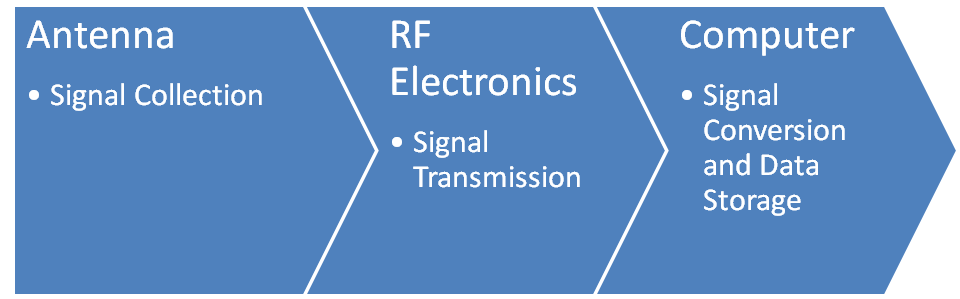
\includegraphics[width=0.9\linewidth]{SCIHI_system/figures/basic_block_diagram.png}
\caption{Basic Block Diagram of the SCI-HI instrument.}
\label{Fig:basic_block_diagram}
\end{center}
\end{figure}

In order to meet these constraints, the instrument design was broken down into three categories based upon their purpose in the overall design (see Figure \ref{Fig:basic_block_diagram}). These categories are an antenna for signal collection, radio frequency (RF) electronics for signal transmission, and a computer for signal processing and storage.

\section{Antenna}
When designing an instrument for radio astronomy, one of the big challenges is finding an antenna design that fits the particular needs of a given experiment. 

\subsection{Design Considerations}
For the SCI-HI experiment, the key properties for the antenna selection were the bandwidth and stability of the antenna beam pattern and impedance (S-parameters) over frequency. 

\textcolor{red}{Here I will add a brief discussion of antenna design including some of the key parameters for an antenna in general and why they are significant. }

\begin{figure}[htb]
\centering
\begin{minipage}[b]{0.45\textwidth}
\centering
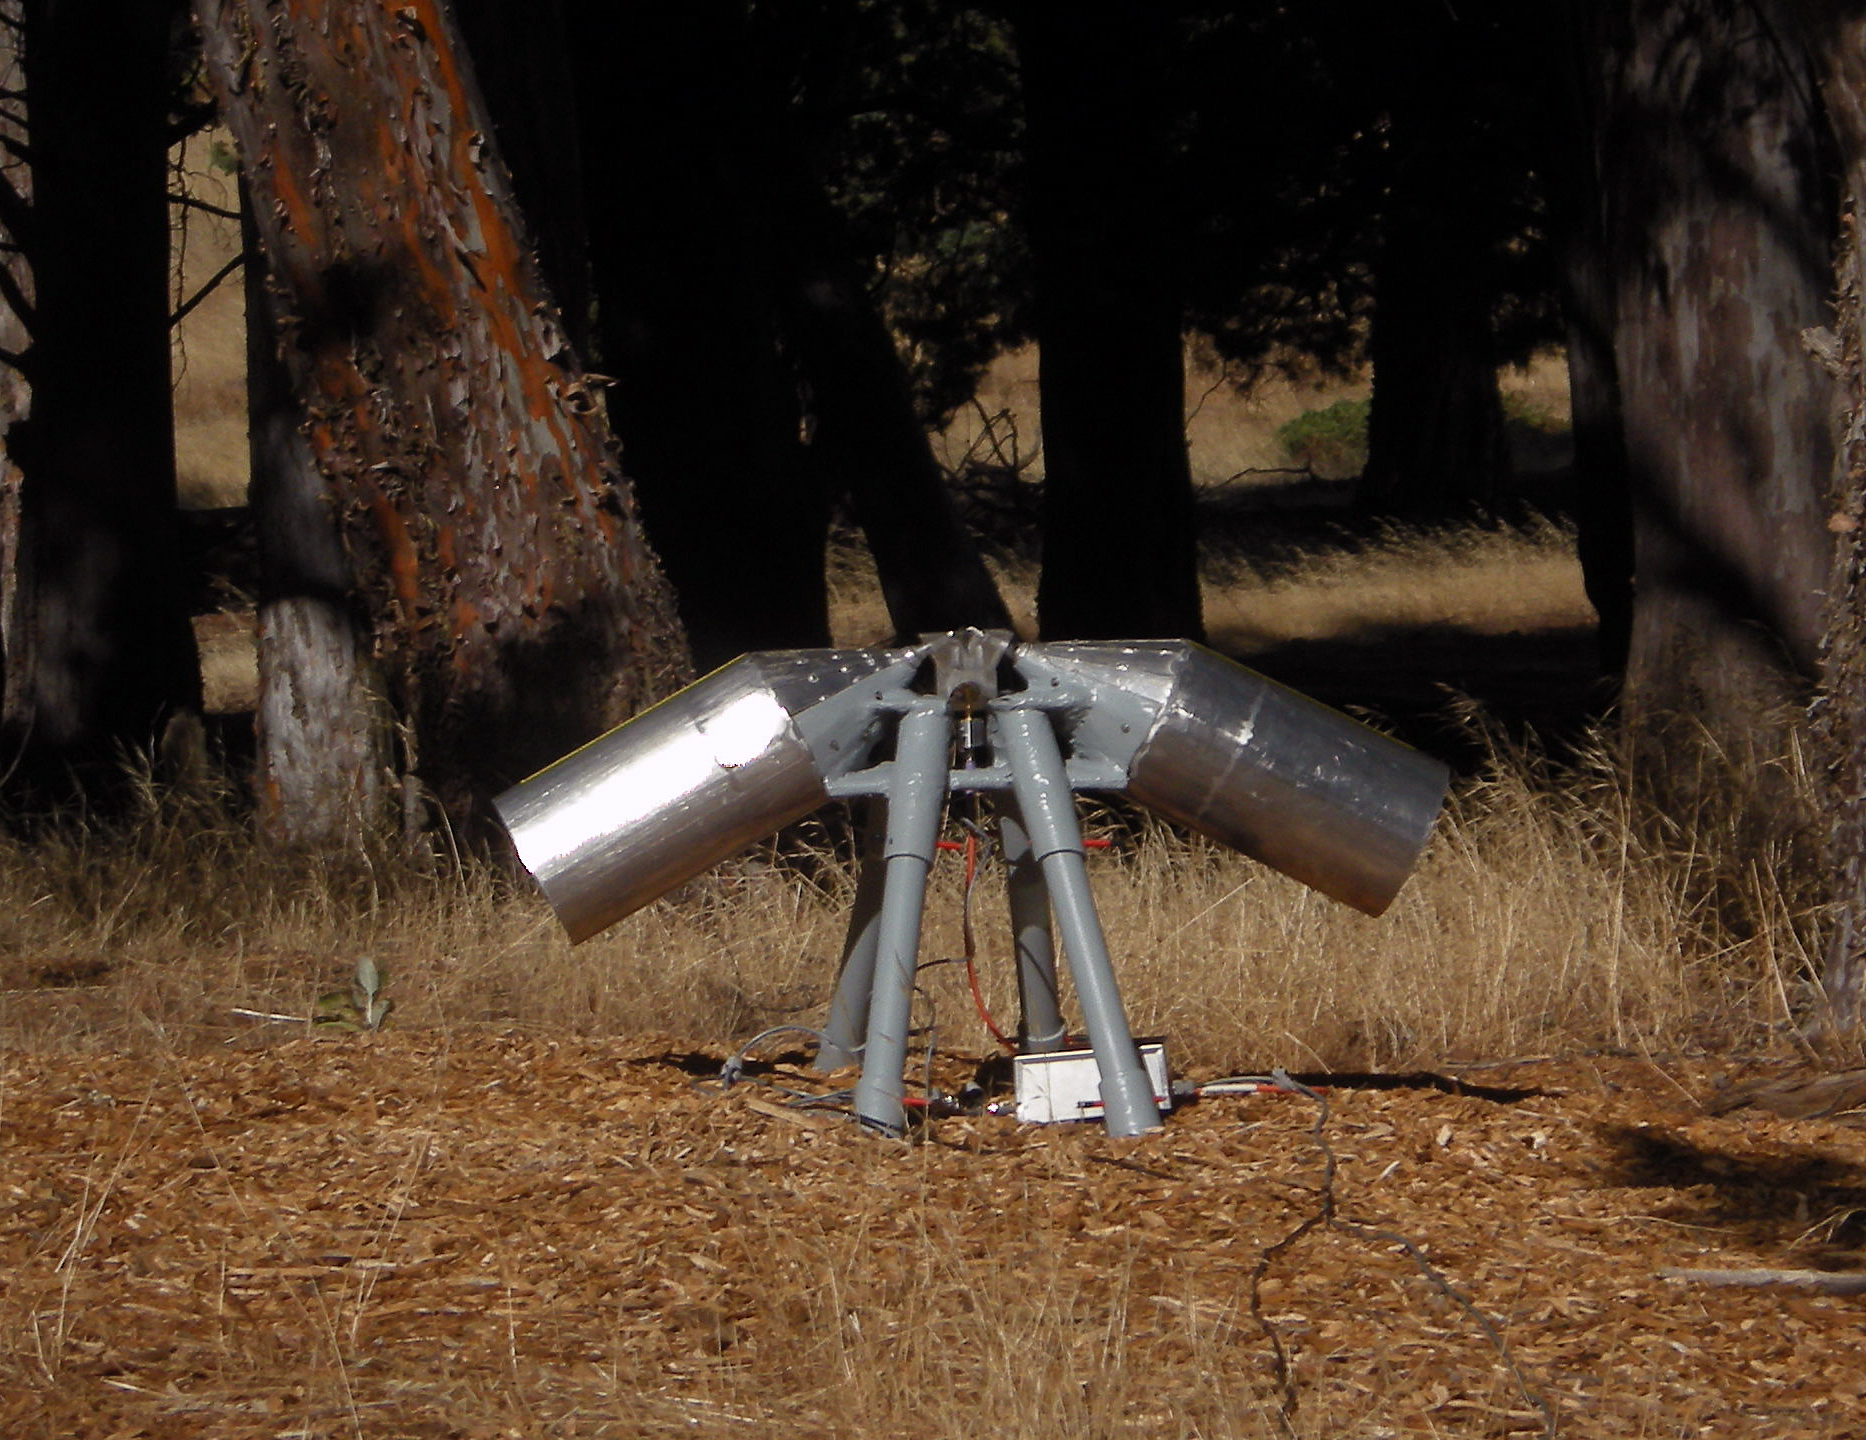
\includegraphics[width=0.95\linewidth]{SCIHI_system/figures/trombone_guad_small.jpg}
\caption{Trombone Antenna setup in its smallest (highest center frequency) configuration.}
\label{Fig:trombone_small}
\end{minipage}%
\begin{minipage}[b]{0.02\textwidth}
\hspace{1cm}
\end{minipage}%
\begin{minipage}[b]{0.51\textwidth}
\centering
\includegraphics[width=0.95\linewidth]{SCIHI_system/figures/trombone_pgh_zoom.jpg}
\caption{Trombone Antenna setup in its largest (lowest center frequency) configuration.}
\label{Fig:trombone_large}
\end{minipage}
\end{figure}

\subsection{First Stage Antenna}
Initially, we started with a simple $''$Trombone$''$ antenna. This design is a dipole with fat, angled elements over a ground plane (see Figures \ref{Fig:trombone_small} and \ref{Fig:trombone_large}). Changing the frequency range of the antenna simply required shifting the length of the dipole elements and their position above the ground plane. 

\begin{figure}[htb]
\centering
\begin{minipage}[b]{0.53\textwidth}
\centering
\includegraphics[width=0.95\linewidth]{SCIHI_system/figures/trombone_mount.jpg}
\caption{Mounting for the Trombone antenna, with lucite mount point and fiberglass support structure. }
\label{Fig:trombone_mount}
\end{minipage}%
\begin{minipage}[b]{0.02\textwidth}
\hspace{1cm}
\end{minipage}%
\begin{minipage}[b]{0.41\textwidth}
\centering
\includegraphics[width=0.95\linewidth]{SCIHI_system/figures/trombone_guad_adj.jpg}
\caption{Changing the Trombone antenna configuration from small to large.}
\label{Fig:trombone_adj}
\end{minipage}
\end{figure}

\subsubsection{Antenna Construction}
The trombone shapes were constructed out of welded aluminum with a lucite mounting block at the connection point of the two cones (see Figure \ref{Fig:trombone_mount}), The dipoles and mounting block were supported with a structure constructed out of fiberglass and PVC tubes. The entire system was placed above a ground plane composed of metal mesh (aka chicken wire) over a small ($\sim9 m^2$) area and long wire extensions ($\sim10 m$) extending out from the center like a spider web. 

Tuning the trombone length was accomplished with an external tube that slid over the main dipole elements (see Figure \ref{Fig:trombone_adj}), while adjusting the height of the trombone was done using the support legs (PVC pipes with variable heights).

The Trombone antenna was used throughout the initial stages of the SCI-HI project, including deployments at Green Bank in West Virginia (Figure \ref{Fig:trombone_gbt}), the Zona del Silencio in Mexico (Figure \ref{Fig:trombone_zds}), Algonquin Radio Observatory in Canada (Figure \ref{Fig:trombone_alg}), and Isla Guadalupe in Mexico (Figure \ref{Fig:trombone_guad}). For more discussion of these sites, see Chapter \ref{Ch:RFI}.

\begin{figure}[htb]
\centering
\begin{minipage}[b]{0.48\textwidth}
\centering
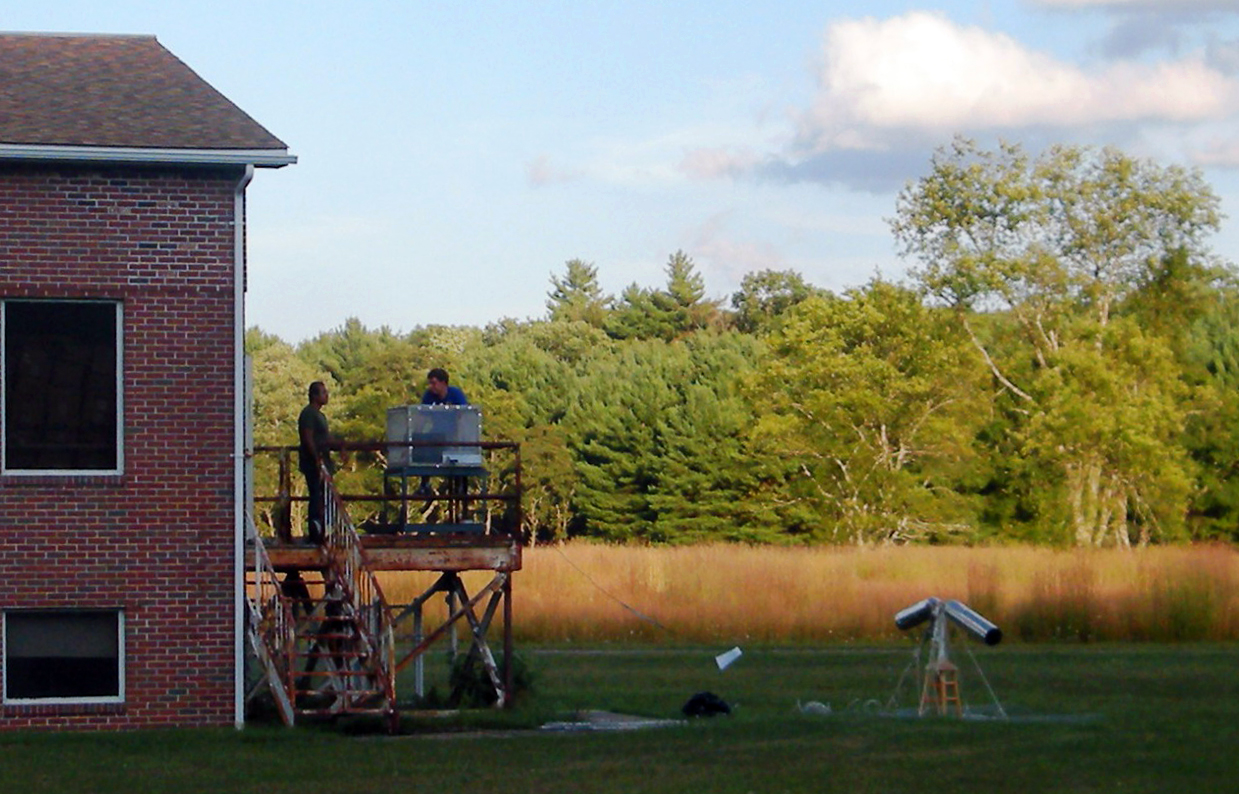
\includegraphics[width=0.95\linewidth]{SCIHI_system/figures/trombone_gbt.jpg}
\caption{SCI-HI setup with trombone antenna on site at Green Bank in August 2011.}
\label{Fig:trombone_gbt}
\end{minipage}%
\begin{minipage}[b]{0.02\textwidth}
\hspace{1cm}
\end{minipage}%
\begin{minipage}[b]{0.46\textwidth}
\centering
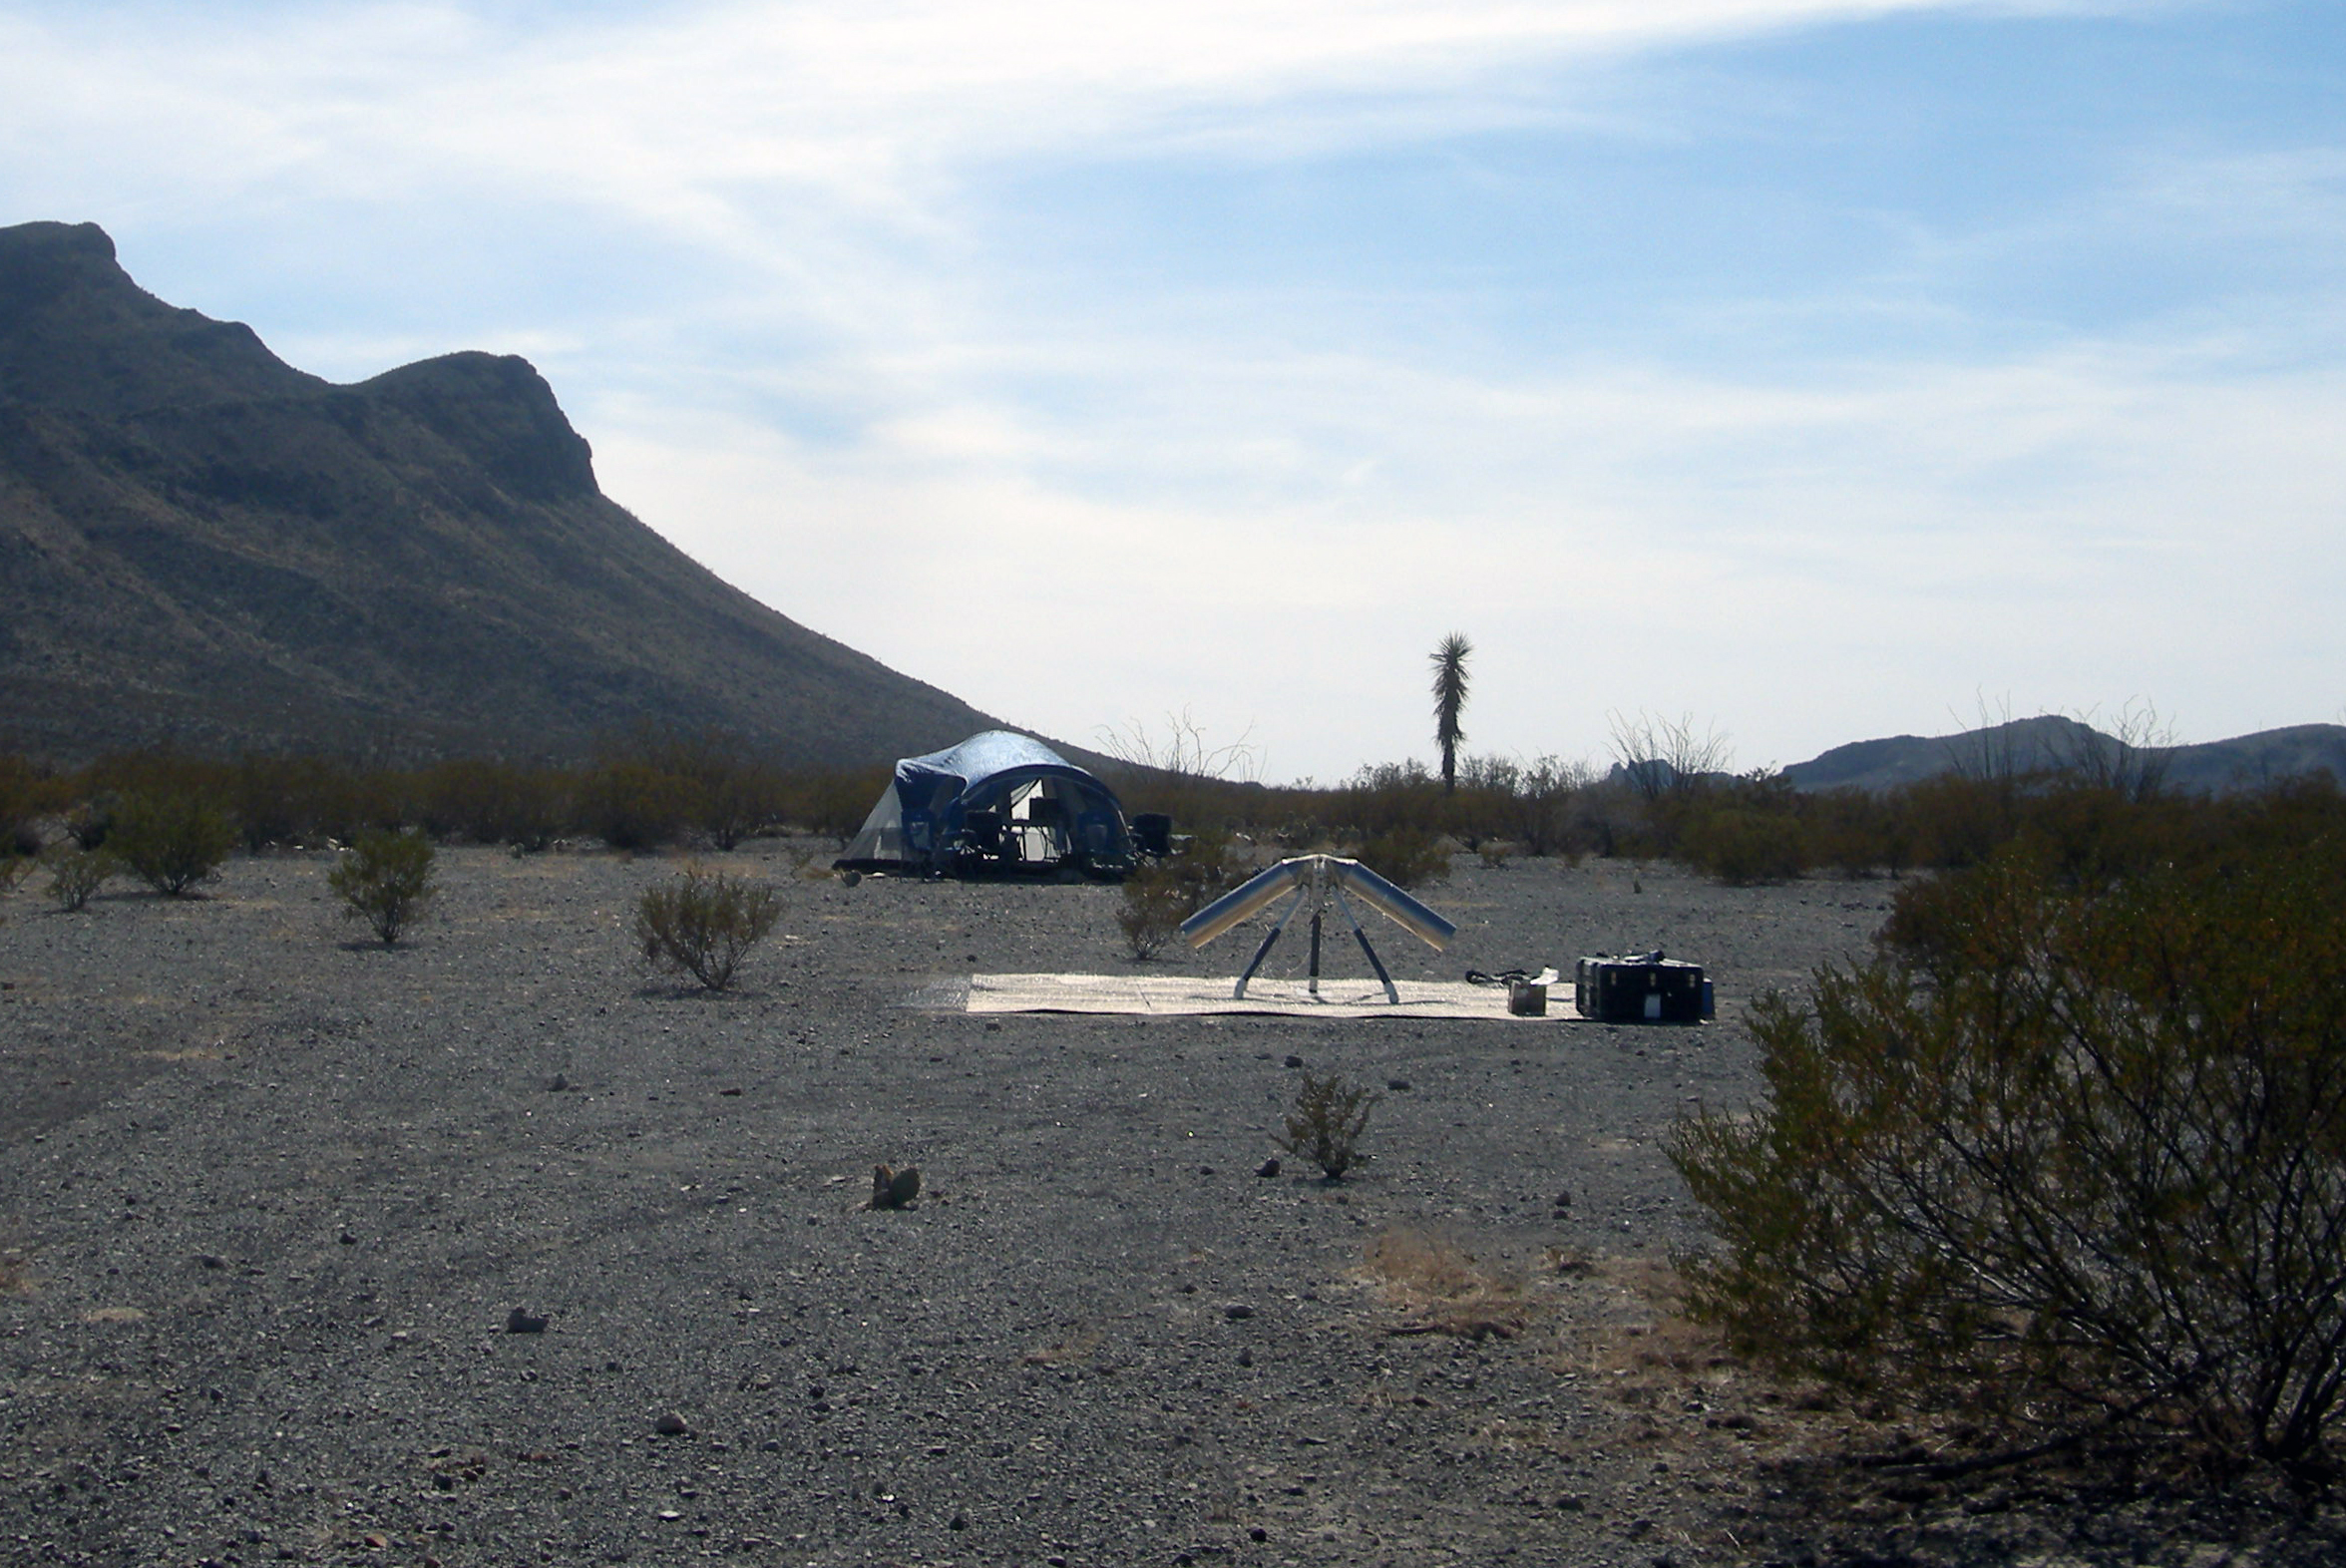
\includegraphics[width=0.95\linewidth]{SCIHI_system/figures/trombone_sys_ZdS.jpg}
\caption{SCI-HI setup with trombone antenna on site at the Zona del Silencio in January 2012.}
\label{Fig:trombone_zds}
\end{minipage}
\end{figure}

\begin{figure}[htb]
\centering
\begin{minipage}[b]{0.52\textwidth}
\centering
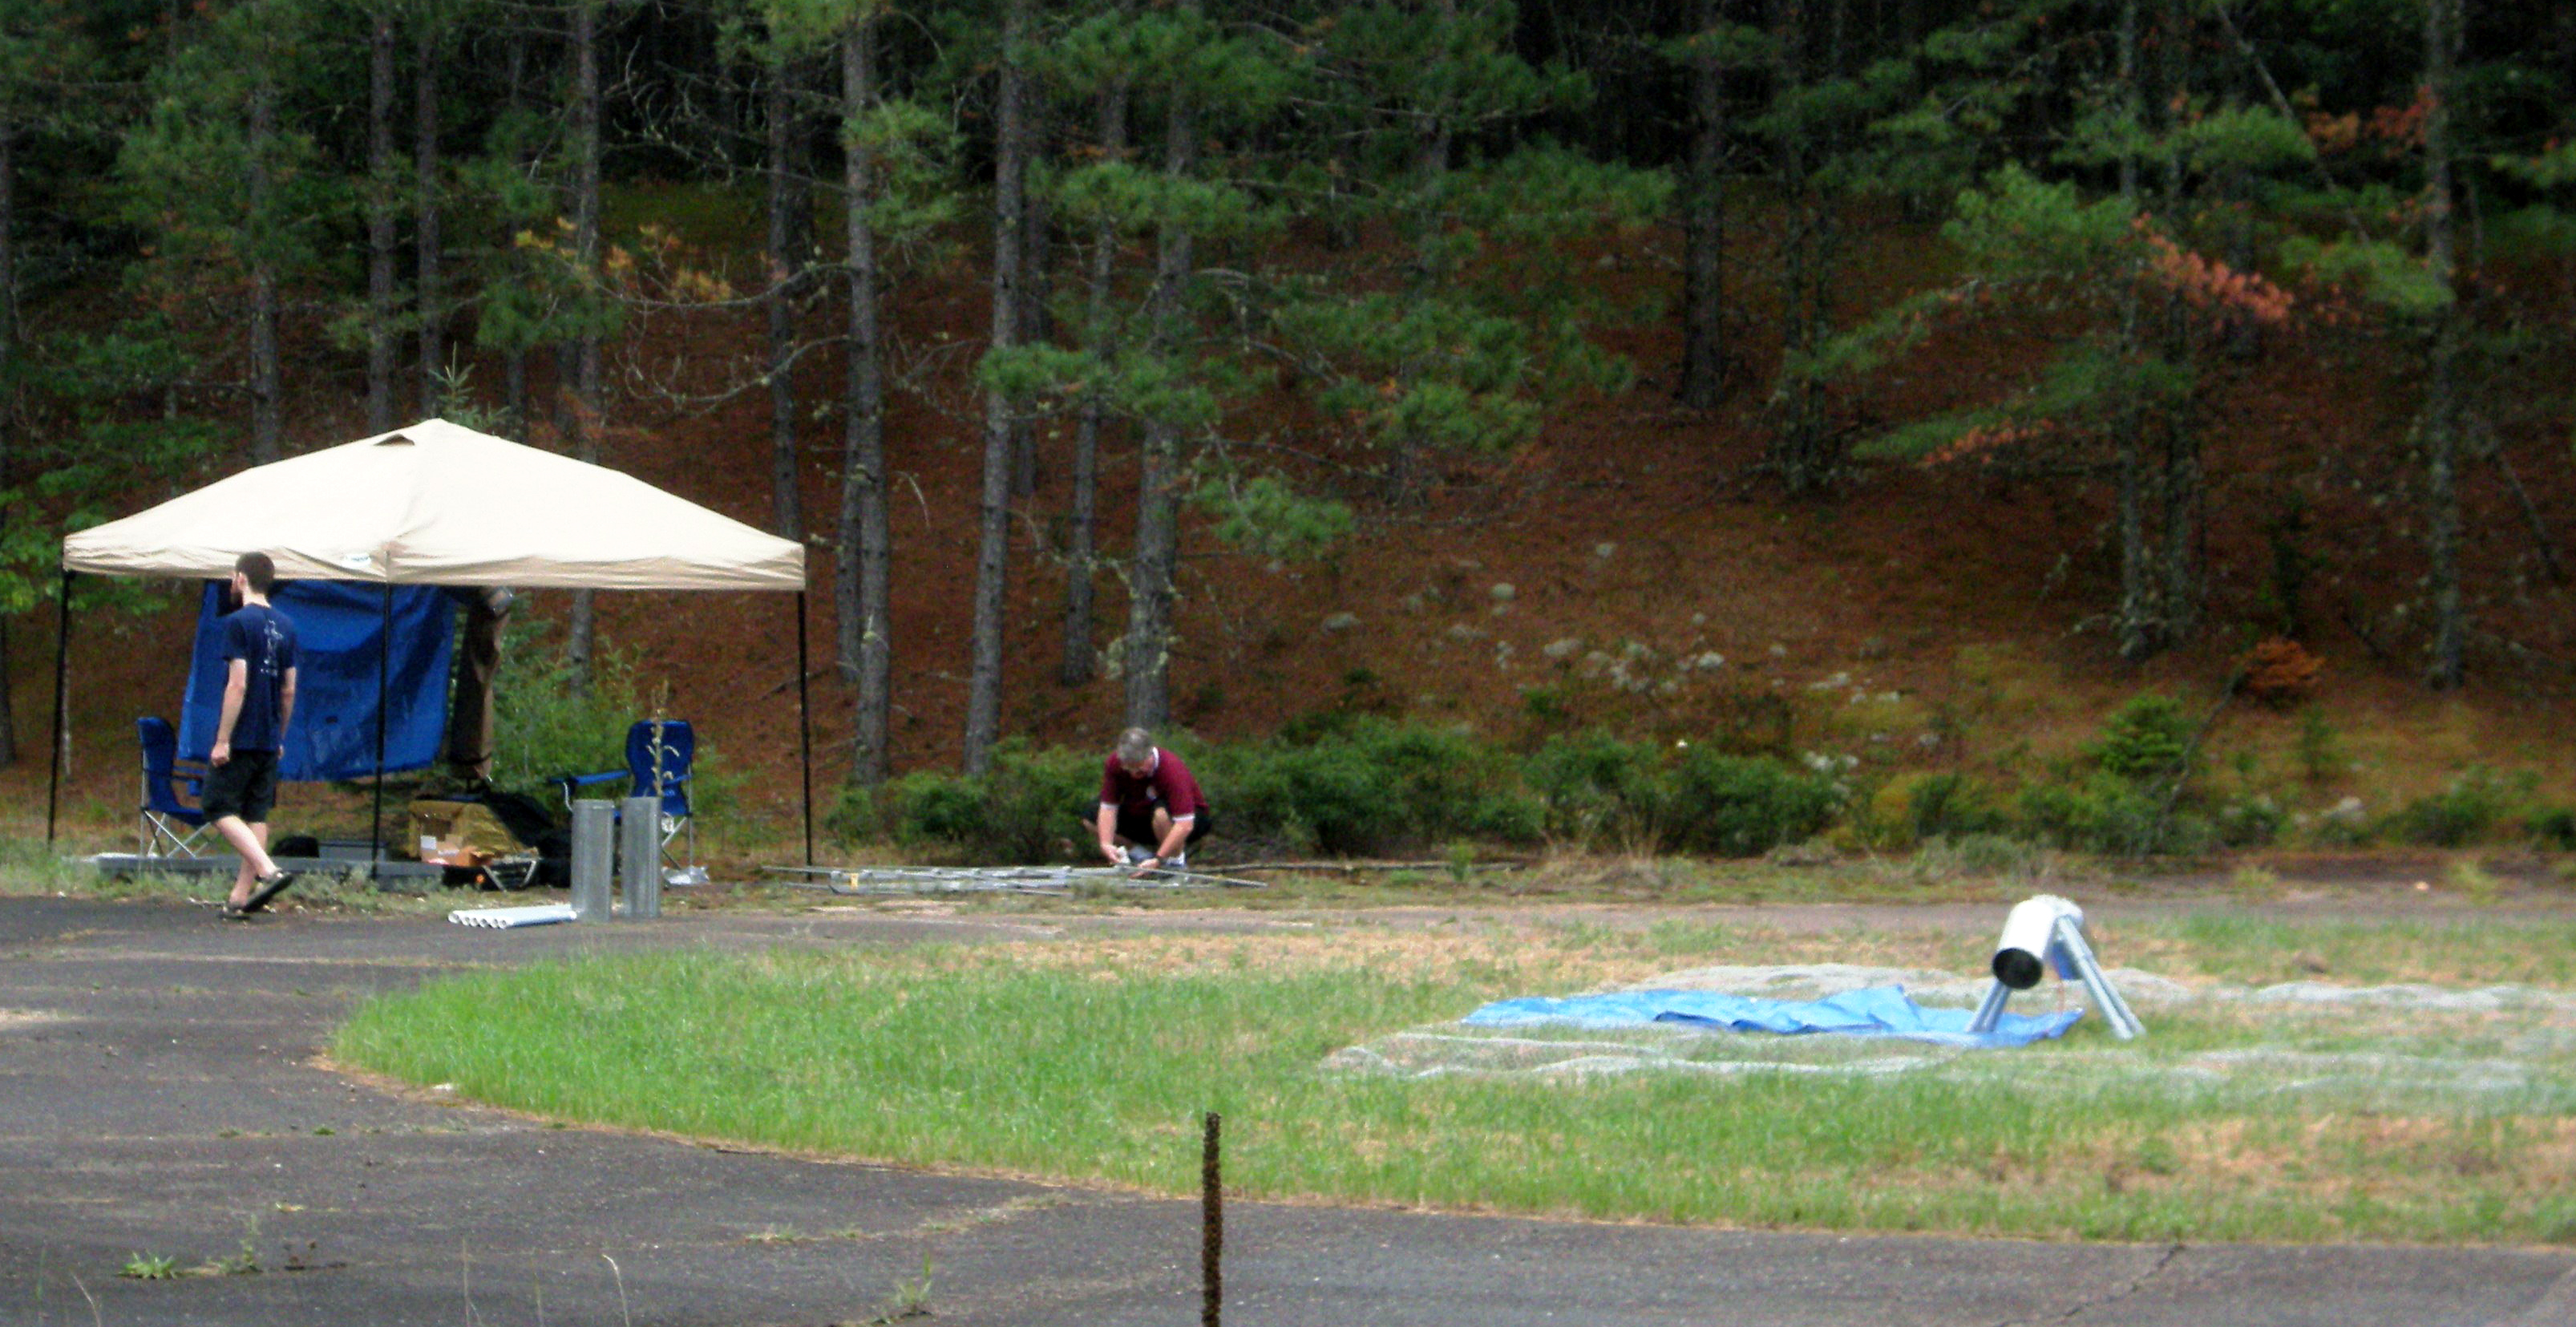
\includegraphics[width=0.95\linewidth]{SCIHI_system/figures/trombone_alg_sys.jpg}
\caption{SCI-HI setup with trombone antenna on site at the Algonquin Radio Observatory in August 2012.}
\label{Fig:trombone_alg}
\end{minipage}%
\begin{minipage}[b]{0.02\textwidth}
\hspace{1cm}
\end{minipage}%
\begin{minipage}[b]{0.42\textwidth}
\centering
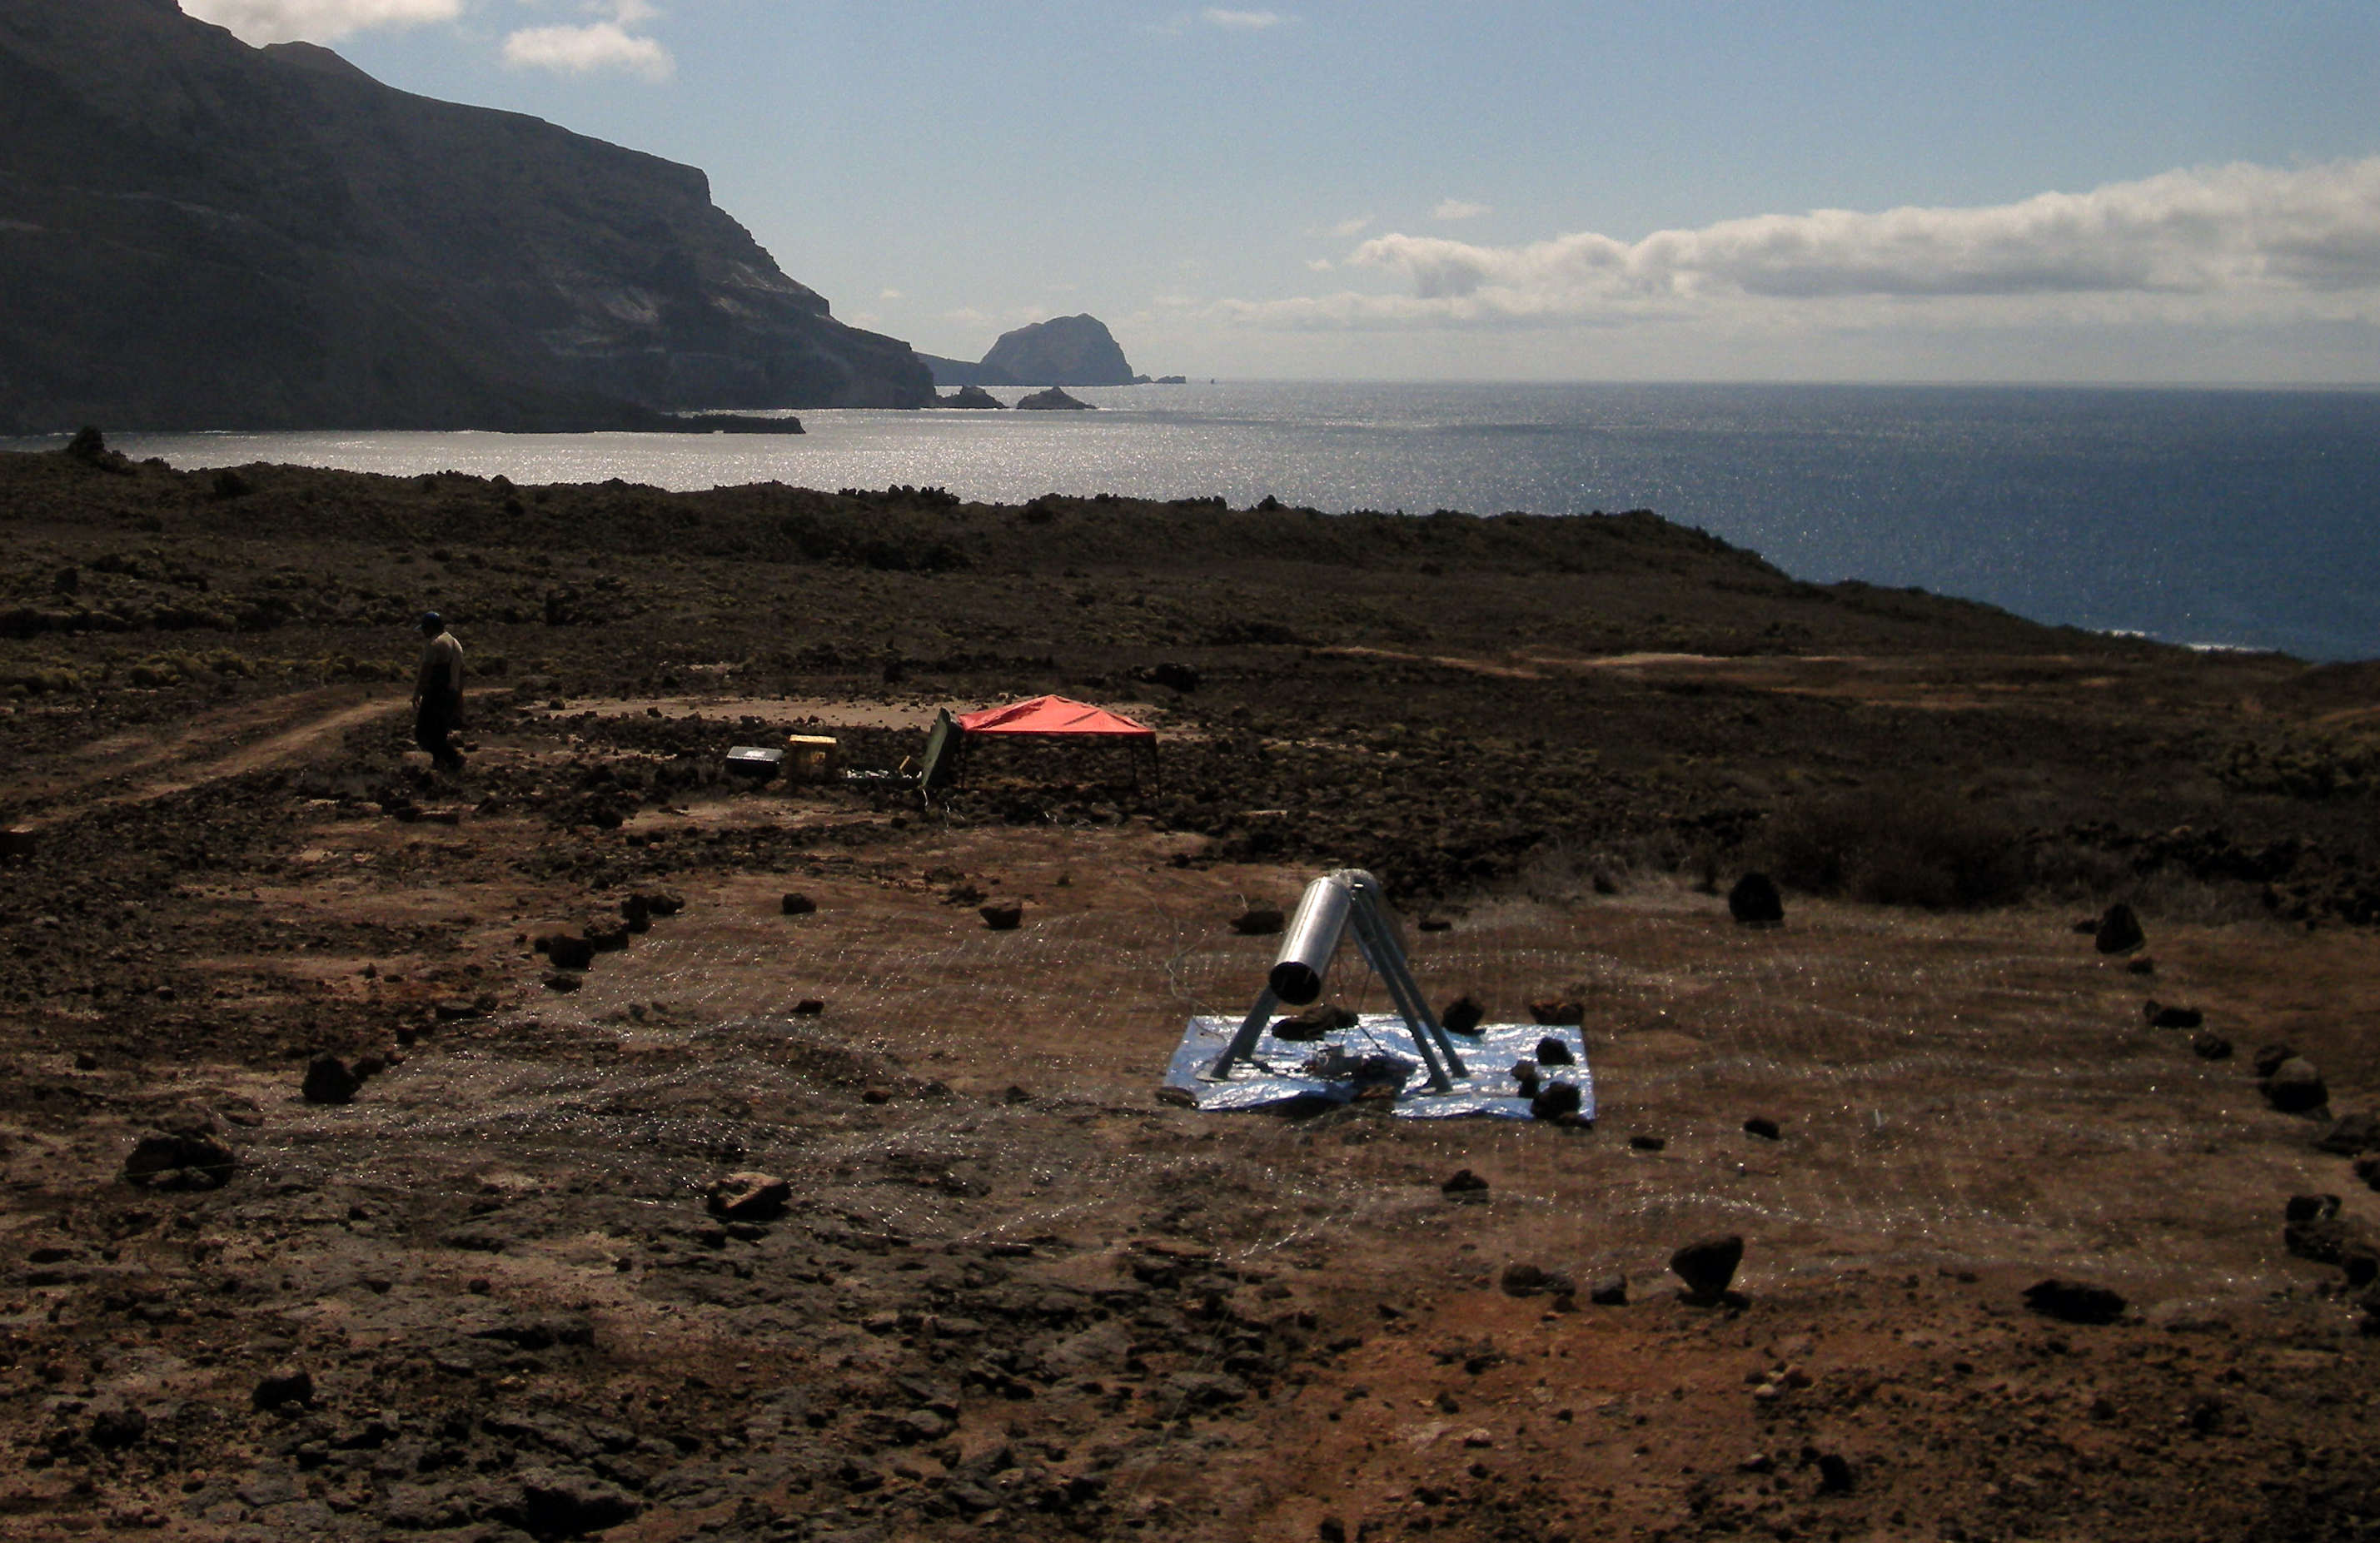
\includegraphics[width=0.95\linewidth]{SCIHI_system/figures/trombone_sys_guad.jpg}
\caption{SCI-HI setup with trombone antenna on site at Isla Guadalupe in October 2012.}
\label{Fig:trombone_guad}
\end{minipage}
\end{figure}

\subsubsection{Antenna Simulation}
Simulating the Trombone antenna indicated some problems with the design, including significant structure in the antenna beam and S-parameters. \textcolor{red}{Add image/details of Amy's simulation results.}

\subsection{HIbiscus Antenna Design}

Because of the problems we had with the trombone design, we decided to shift our antenna design in a new direction based upon our expectations from the literature (\textcolor{red}{Need to add specific references for different antenna types}). We tested several antenna designs in simulation, including the four-square design used in the EDGES experiment \cite{rogers_2012}. This testing was done using FEKO, a finite element computational electromagnetics software package.\footnote{https://www.feko.info/}

Based on the FEKO simulation results we settled on a design that used the EDGES design as a starting point, but changed the exact shapes of the four squares. We took each square and turned it into an incliclined petal composed of three trapezoidal shapes. Each shape was connected to its neighbors on the petal, but had a different angle with respect to the ground. Additional panels were added to each side of the petal to create a strip line with a fixed gap between the petals. The entire antenna was then placed a distance above a flat ground plane. We call this design a HIbiscus antenna. 

\textcolor{red}{Add either pictures or simulation images for antenna shape details.}

We found that the shape parameters that were most significant in affecting antenna performance were the strip line gap width and the height of the antenna with respect to the ground plane. 


\begin{figure}[htb]
\centering
\begin{minipage}[b]{0.50\textwidth}
\centering
\includegraphics[width=0.95\linewidth]{SCIHI_system/figures/model_test_tabitha.jpg}
\caption{Testing a model HIbiscus antenna in the Project REAL Chamber. }
\label{Fig:hibiscus_scale_tabitha}
\end{minipage}%
\begin{minipage}[b]{0.02\textwidth}
\hspace{1cm}
\end{minipage}%
\begin{minipage}[b]{0.44\textwidth}
\centering
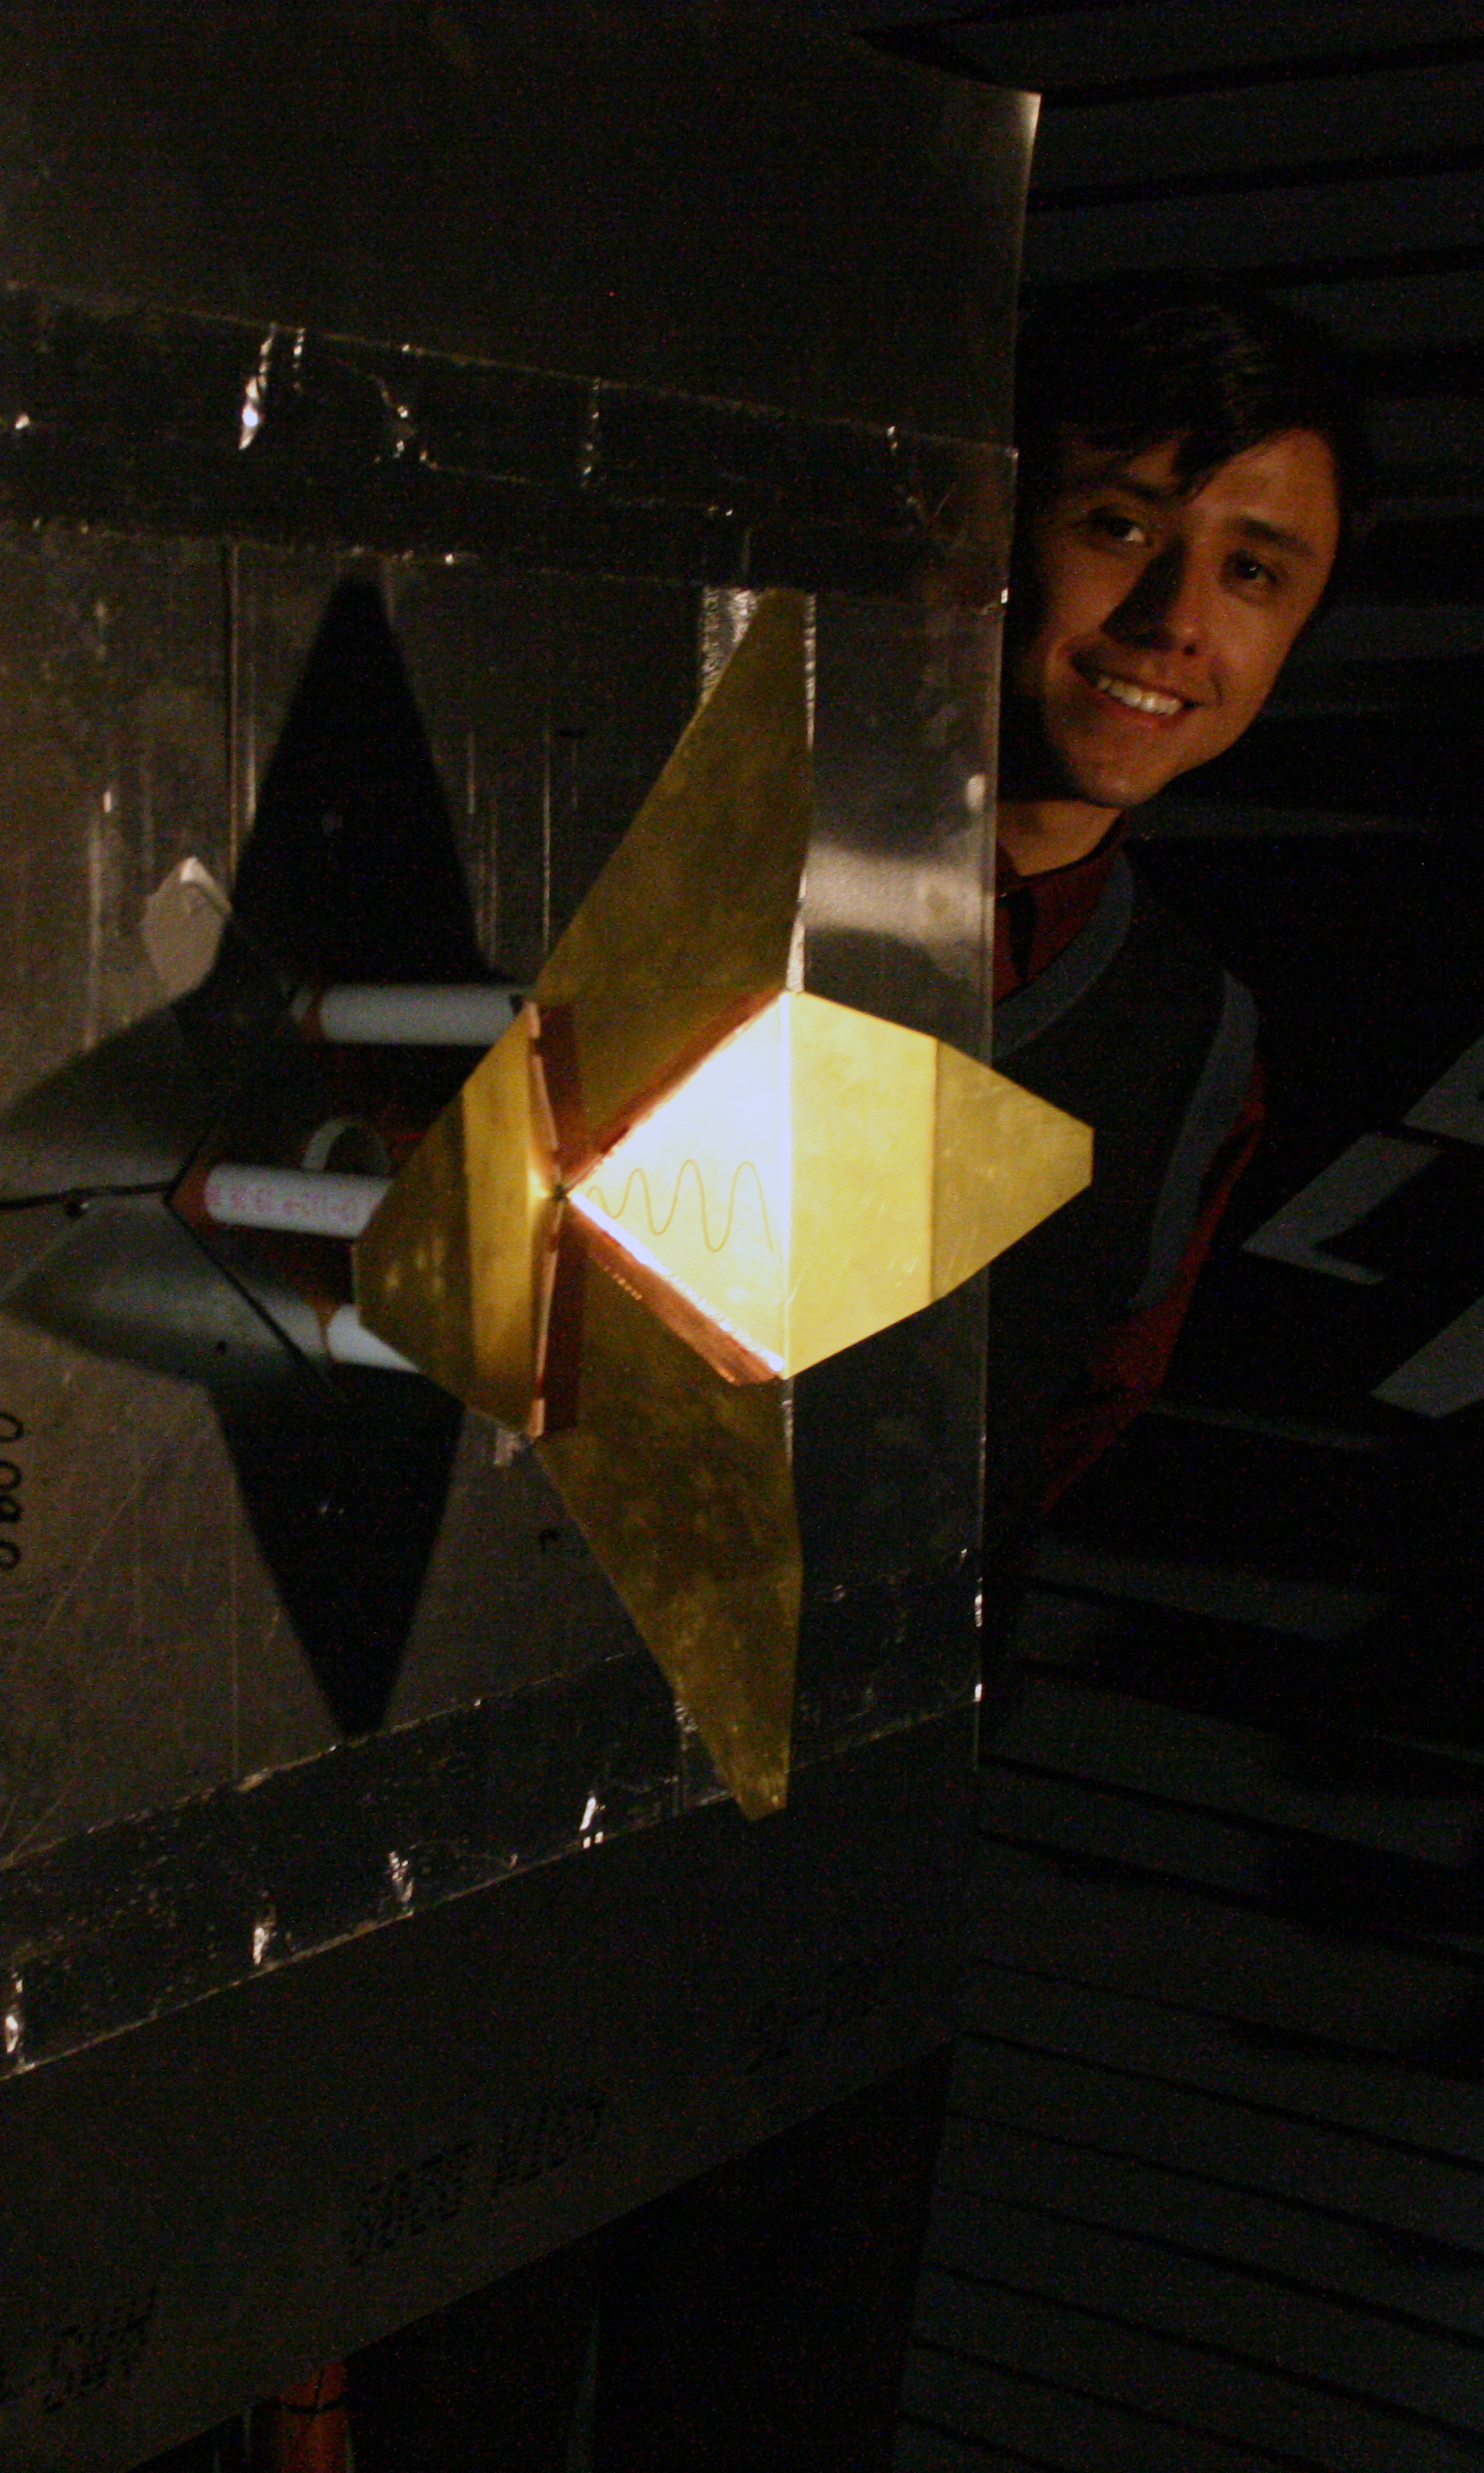
\includegraphics[width=0.95\linewidth]{SCIHI_system/figures/model_test_jose.jpg}
\caption{Scale model test with a different HIbiscus antenna model.}
\label{Fig:hibiscus_scale_jose}
\end{minipage}
\end{figure}

\subsubsection{Scale Model Testing}
In order to test our simulation to see if it matched the real antenna performance, we built a set of scaled HIbiscus designs tuned for higher frequencies around 400 MHz. This allowed us to use an antenna range to measure the antenna beam shape and s-parameters. 

We used the Project REAL\footnote{http://www.preal.ece.cmu.edu/} (Remote Educational Antenna Laboratory) facility at Carnegie Mellon University to measure the antenna response of different scaled HIbiscus models, as is shown in Figures \ref{Fig:hibiscus_scale_tabitha} and \ref{Fig:hibiscus_scale_jose}. By incrementally adjusting the strip line gap width and antenna height we were able to tune the antenna scale model to optimize these critical parameters in a real design. 

Using the scale model data, we were also able to edit the antenna simulation to better match the actual antenna response, providing us with an antenna simulation dataset that was closer to reality. 

\textcolor{red}{Here there will be some paragraphs about the exact simulation and scale model measurements including plots of impedence and antenna pattern.}

\begin{figure}[htb]
\centering
\begin{minipage}[b]{0.43\textwidth}
\centering
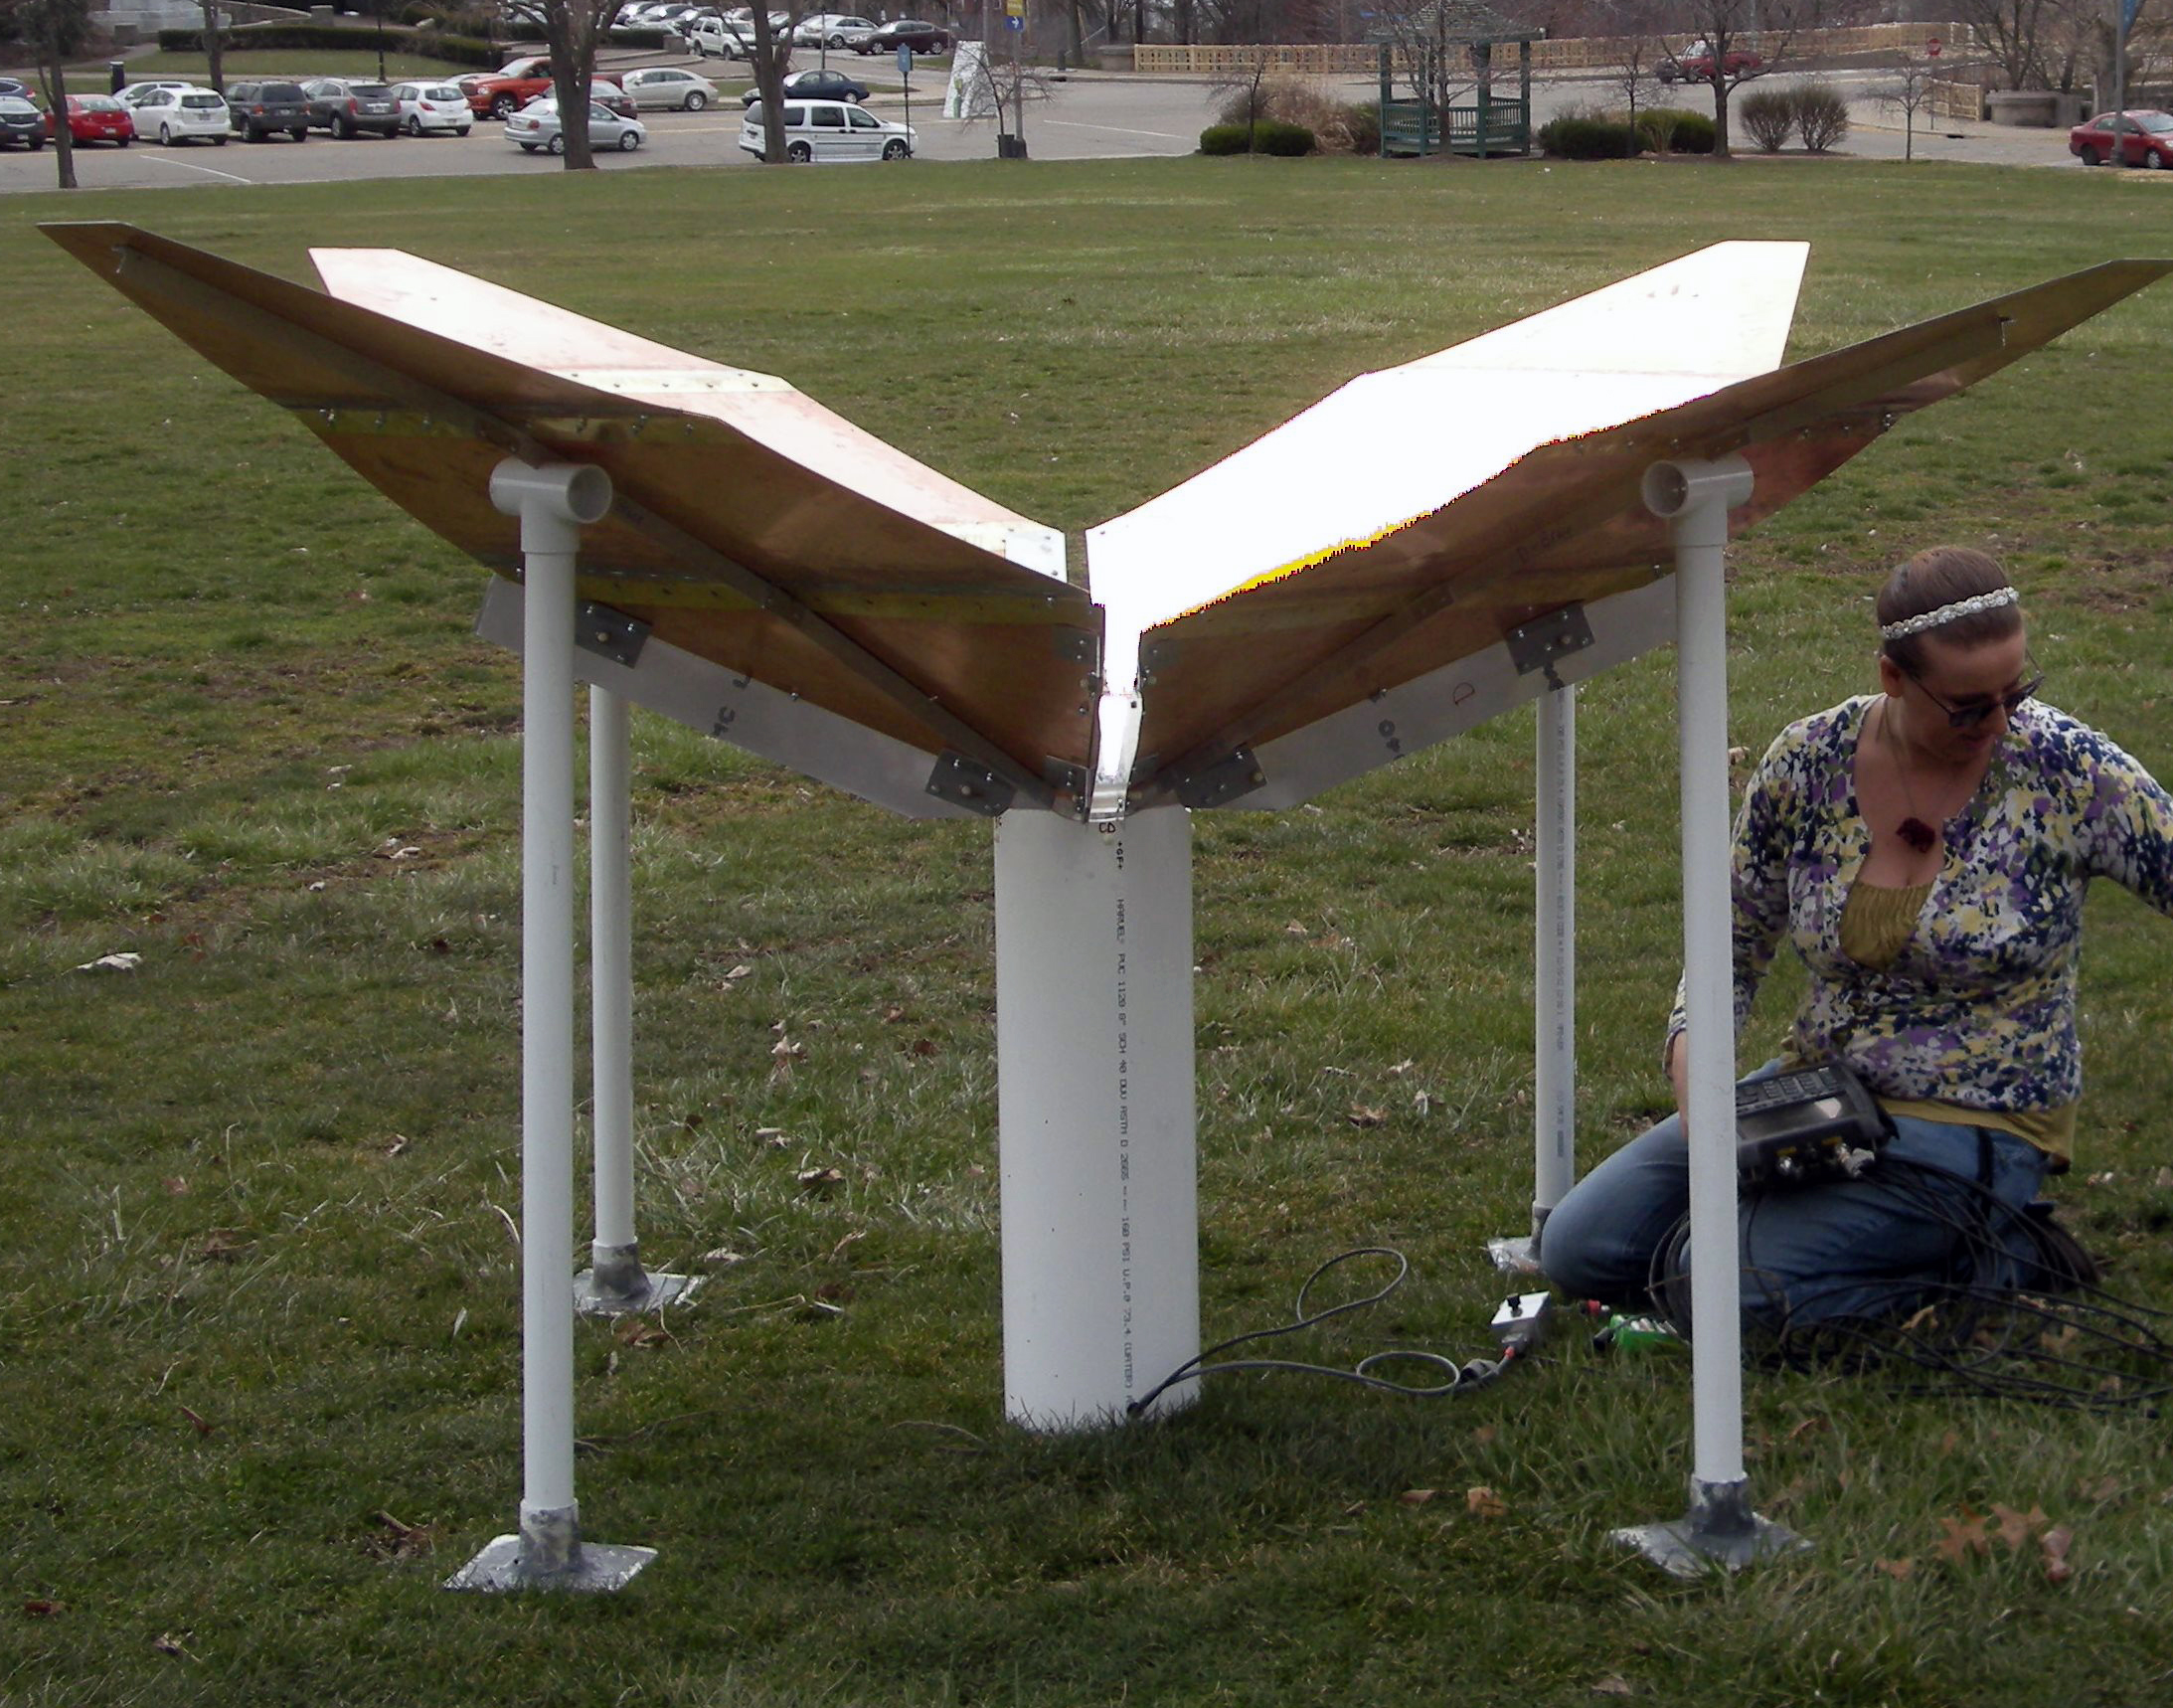
\includegraphics[width=0.95\linewidth]{SCIHI_system/figures/HIbiscus_pgh_imp.jpg}
\caption{HIbiscus antenna scaled for 70 MHz as it was setup during s-parameter testing at CMU. }
\label{Fig:hibiscus_first}
\end{minipage}%
\begin{minipage}[b]{0.02\textwidth}
\hspace{1cm}
\end{minipage}%
\begin{minipage}[b]{0.51\textwidth}
\centering
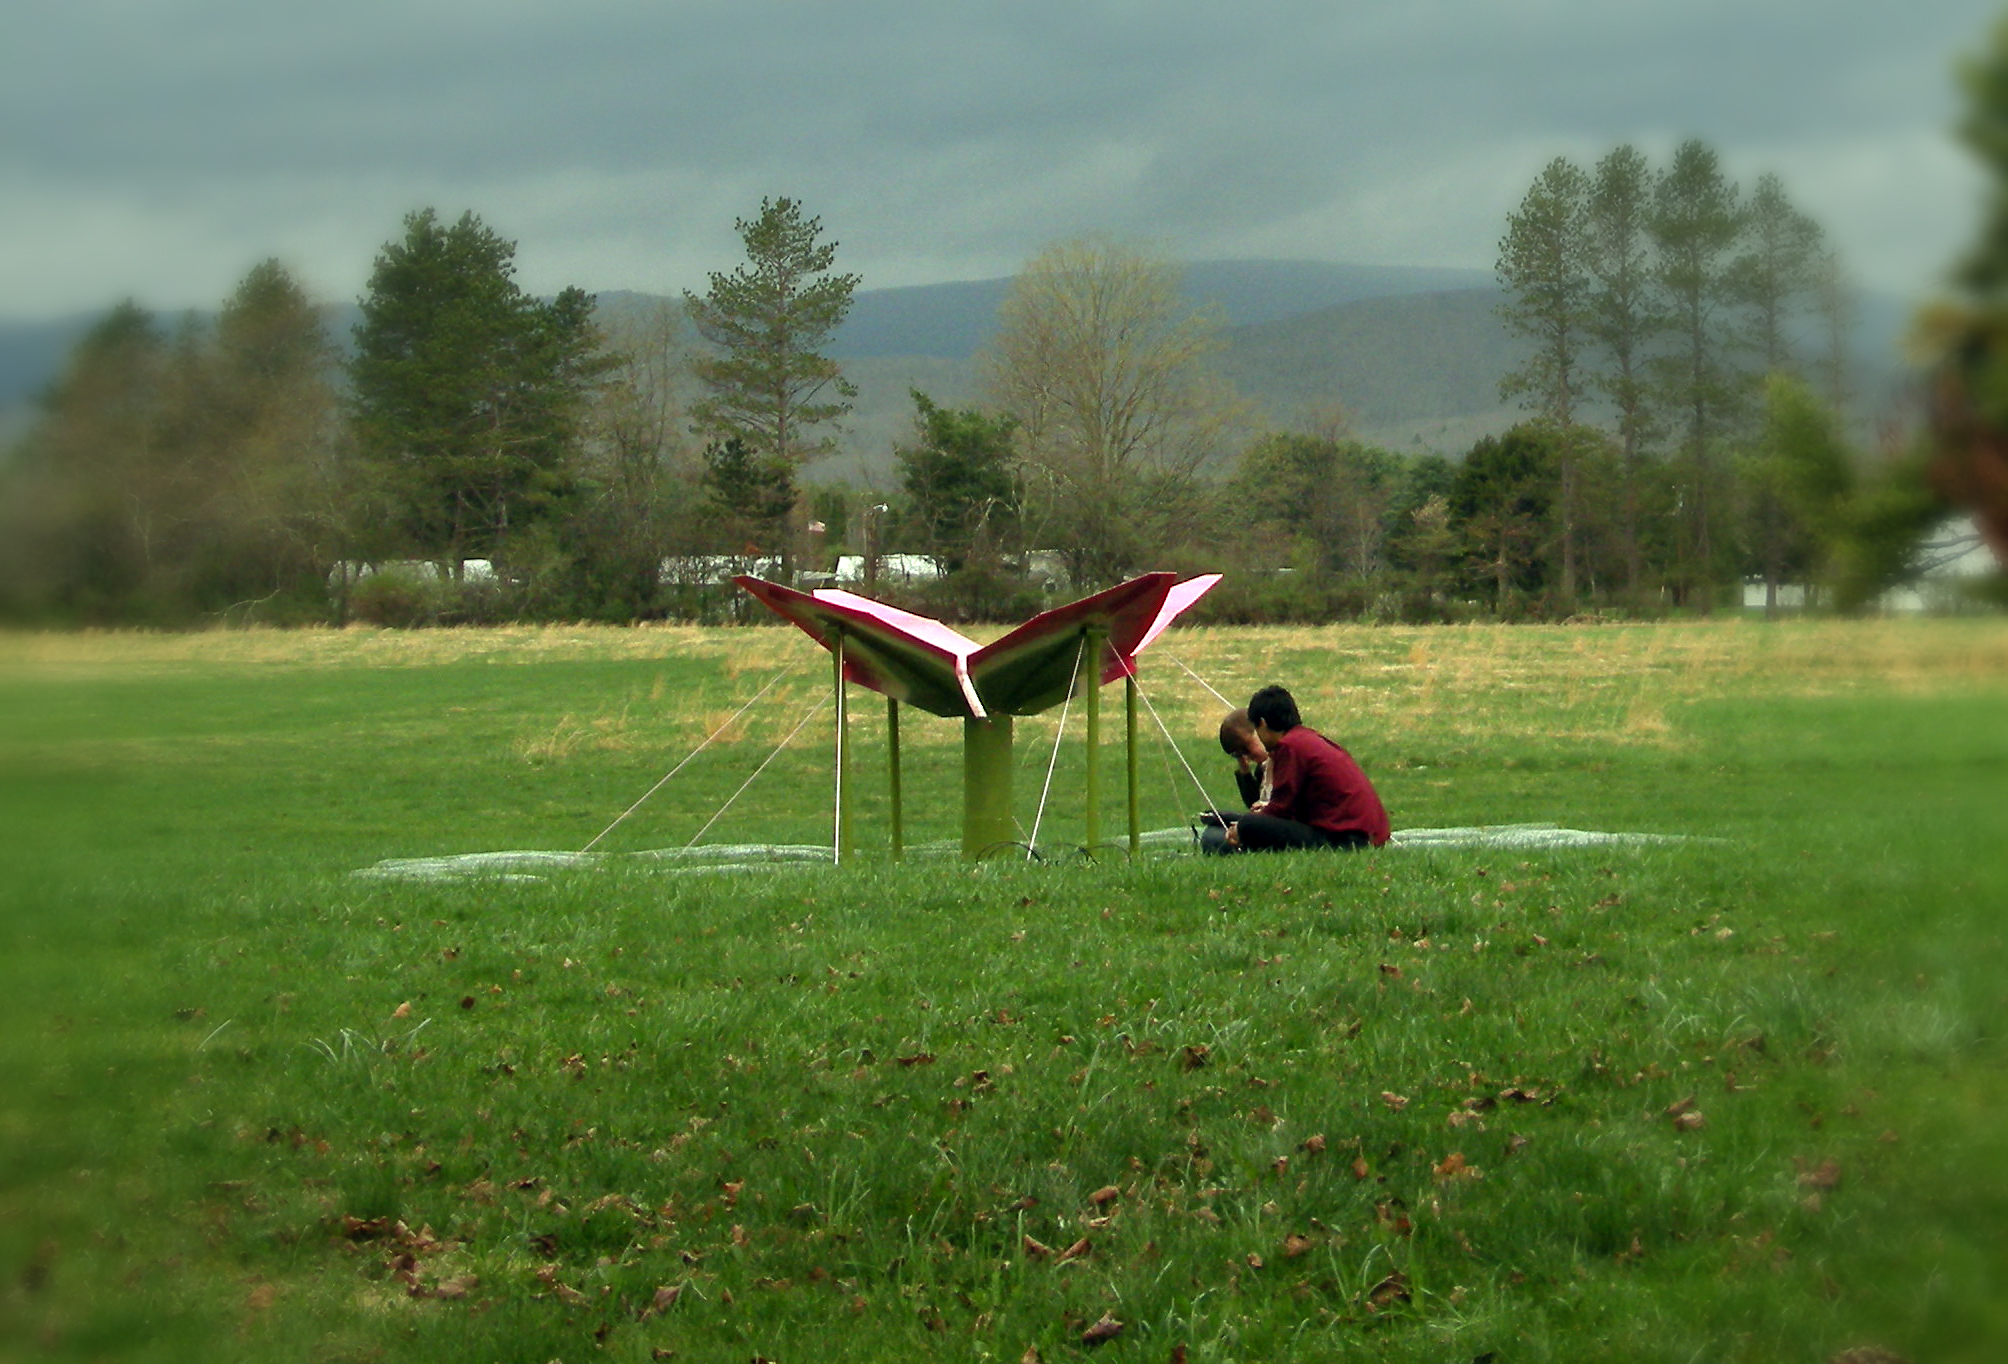
\includegraphics[width=0.95\linewidth]{SCIHI_system/figures/HIbiscus_gbt.jpg}
\caption{HIbiscus antenna scaled for 70 MHz setup for s-parameter testing on site at Green Bank.}
\label{Fig:hibiscus_gbt}
\end{minipage}
\end{figure}

\subsection{HIbiscus Antenna Construction}

\subsubsection{Initial Assembly}
Once we had a design finalized, we set out to construct a HIbiscus antenna with its center frequency tuned to 70 MHz (in the middle of the SCI-HI observation band).

To construct the antenna petals, we started with large sheets of printed circuit board (pcb) material (see Figure \ref{Fig:hibiscus_pcb}). This material is a sheet of fiberglass sandwiched by two thin sheets of copper. We cut each of the trapezoidal shapes out of the pcb material, then added brass flanges to connect the shapes. Underneath the center line of each petal we placed a rib made out of aluminum angle with the appropriate bends to match the angles between trapezoids. Finally, the strip line panels were added using aluminum sheets soldered to some of the trapezoids (see Figure \ref{Fig:hibiscus_solder}). The entire system is bolted together using screws, and can be separated into parts for travel. 

\begin{figure}[htb]
\centering
\begin{minipage}[b]{0.39\textwidth}
\centering
\includegraphics[width=0.95\linewidth]{SCIHI_system/figures/HIbiscus_pcb_cut.jpg}
\caption{HIbiscus antenna pcb panels being cut. }
\label{Fig:hibiscus_pcb}
\end{minipage}%
\begin{minipage}[b]{0.02\textwidth}
\hspace{1cm}
\end{minipage}%
\begin{minipage}[b]{0.55\textwidth}
\centering
\includegraphics[width=0.95\linewidth]{SCIHI_system/figures/HIbiscus_solder.jpg}
\caption{Soldering the strip line to the HIbiscus antenna panels.}
\label{Fig:hibiscus_solder}
\end{minipage}
\end{figure} 

In order to keep the petal separation even and correct, lucite spacers were placed between each of the petals (see Figure \ref{Fig:hibiscus_spacer}). In addition, a lucite mount was built for the connection points at the center of the antenna (see Figure \ref{Fig:hibiscus_center}). The entire system was raised above the ground using a set of five PVC pipe legs; a central column and one leg for each petal (see Figure \ref{Fig:hibiscus_first}). 

\begin{figure}[htb]
\centering
\begin{minipage}[b]{0.52\textwidth}
\centering
\includegraphics[width=0.95\linewidth]{SCIHI_system/figures/HIbiscus_strip_line.jpg}
\caption{Sight line down one of the strip lines for the HIbiscus antenna with spacers in place.}
\label{Fig:hibiscus_spacer}
\end{minipage}%
\begin{minipage}[b]{0.02\textwidth}
\hspace{1cm}
\end{minipage}%
\begin{minipage}[b]{0.42\textwidth}
\centering
\includegraphics[width=0.95\linewidth]{SCIHI_system/figures/HIbiscus_center_point.jpg}
\caption{Center of the HIbiscus antenna with spacers and center mount block in place.}
\label{Fig:hibiscus_center}
\end{minipage}
\end{figure}

Beyond the antenna structure, a ground plane was also required to keep the ground pattern constant in time. Like with the Trombone, we used a ground plane made out of chicken wire. In this case, our simulations showed us that a $\sim 100 m^2$ square ground plane was sufficient for our application. The entire system (antenna plus ground plane) was anchored to the ground to minimize the wind impact on the system. Each of the four support legs had an anchoring rope (see Figure \ref{Fig:hibiscus_gbt}), and the chicken wire was also anchored with many stakes. 

With the antenna constructed, we could test that it matched our scale model measurements in terms of its s-parameters. To do this, we set up the antenna outdoors and made measurements with a portable Vector Network Analyzer. Measurements had to be made outdoors because the wavelengths corresponding to the SCI-HI frequencies ($40-130$ MHz) are $\sim$1-10 meters. This large wavelength scale means that reflections from the boundaries of a room can change antenna s-parameters, so accuracy in measurement requires the outdoor setting. Figures \ref{Fig:hibiscus_first} and \ref{Fig:hibiscus_gbt} show examples of how we made this measurement at CMU and Green Bank.

\textcolor{red}{Here I'll add a paragraph with S11 data using VNA and explanation.}

\subsubsection{Travelling with the Antenna}
In order to use the HIbiscus antenna on-site at remote locations, it needed to be transportable to those locations and easily assembled upon arrival. The physical construction of the antenna was designed to match this requirement in a number of ways. 

First, the entire system was made as lightweight as possible. This was accomplished by using the pcb material, which was much lighter and stiffer than the equivalent sheet metal panels would be. 

Second, the system was designed in segments so it could be assembled and disassembled and packed into small bags. Each petal separated out into three trapezoids that were screwed together for assembly, but could be packed as mostly flat sheets. The lucite spacers and mount were attached to the petals using screws and could be removed and packed for travel, as were the PVC pipe supports. 

Third, the entire system was arranged for travel in three suitcases (plus an extra bag for the ground plane chicken wire). These suitcases were small and light enough to be checked as regular baggage on commercial airlines. 

\begin{figure}[htb]
\begin{center}
%\centering
%\begin{minipage}[b]{0.47\textwidth}
%\centering
\includegraphics[width=0.95\linewidth]{SCIHI_system/figures/HIbiscus_70mhz_lab.jpg}
\caption{New HIbiscus antenna scaled for 70 MHz as laid out in the lab. Scale model in picture for comparison.}
\label{Fig:hibiscus_70}
\end{center}
\end{figure}

%\end{minipage}%
%\begin{minipage}[b]{0.02\textwidth}
%\hspace{1cm}
%\end{minipage}%
%\begin{minipage}[b]{0.47\textwidth}
%\centering

\begin{figure}[htb]
\begin{center}
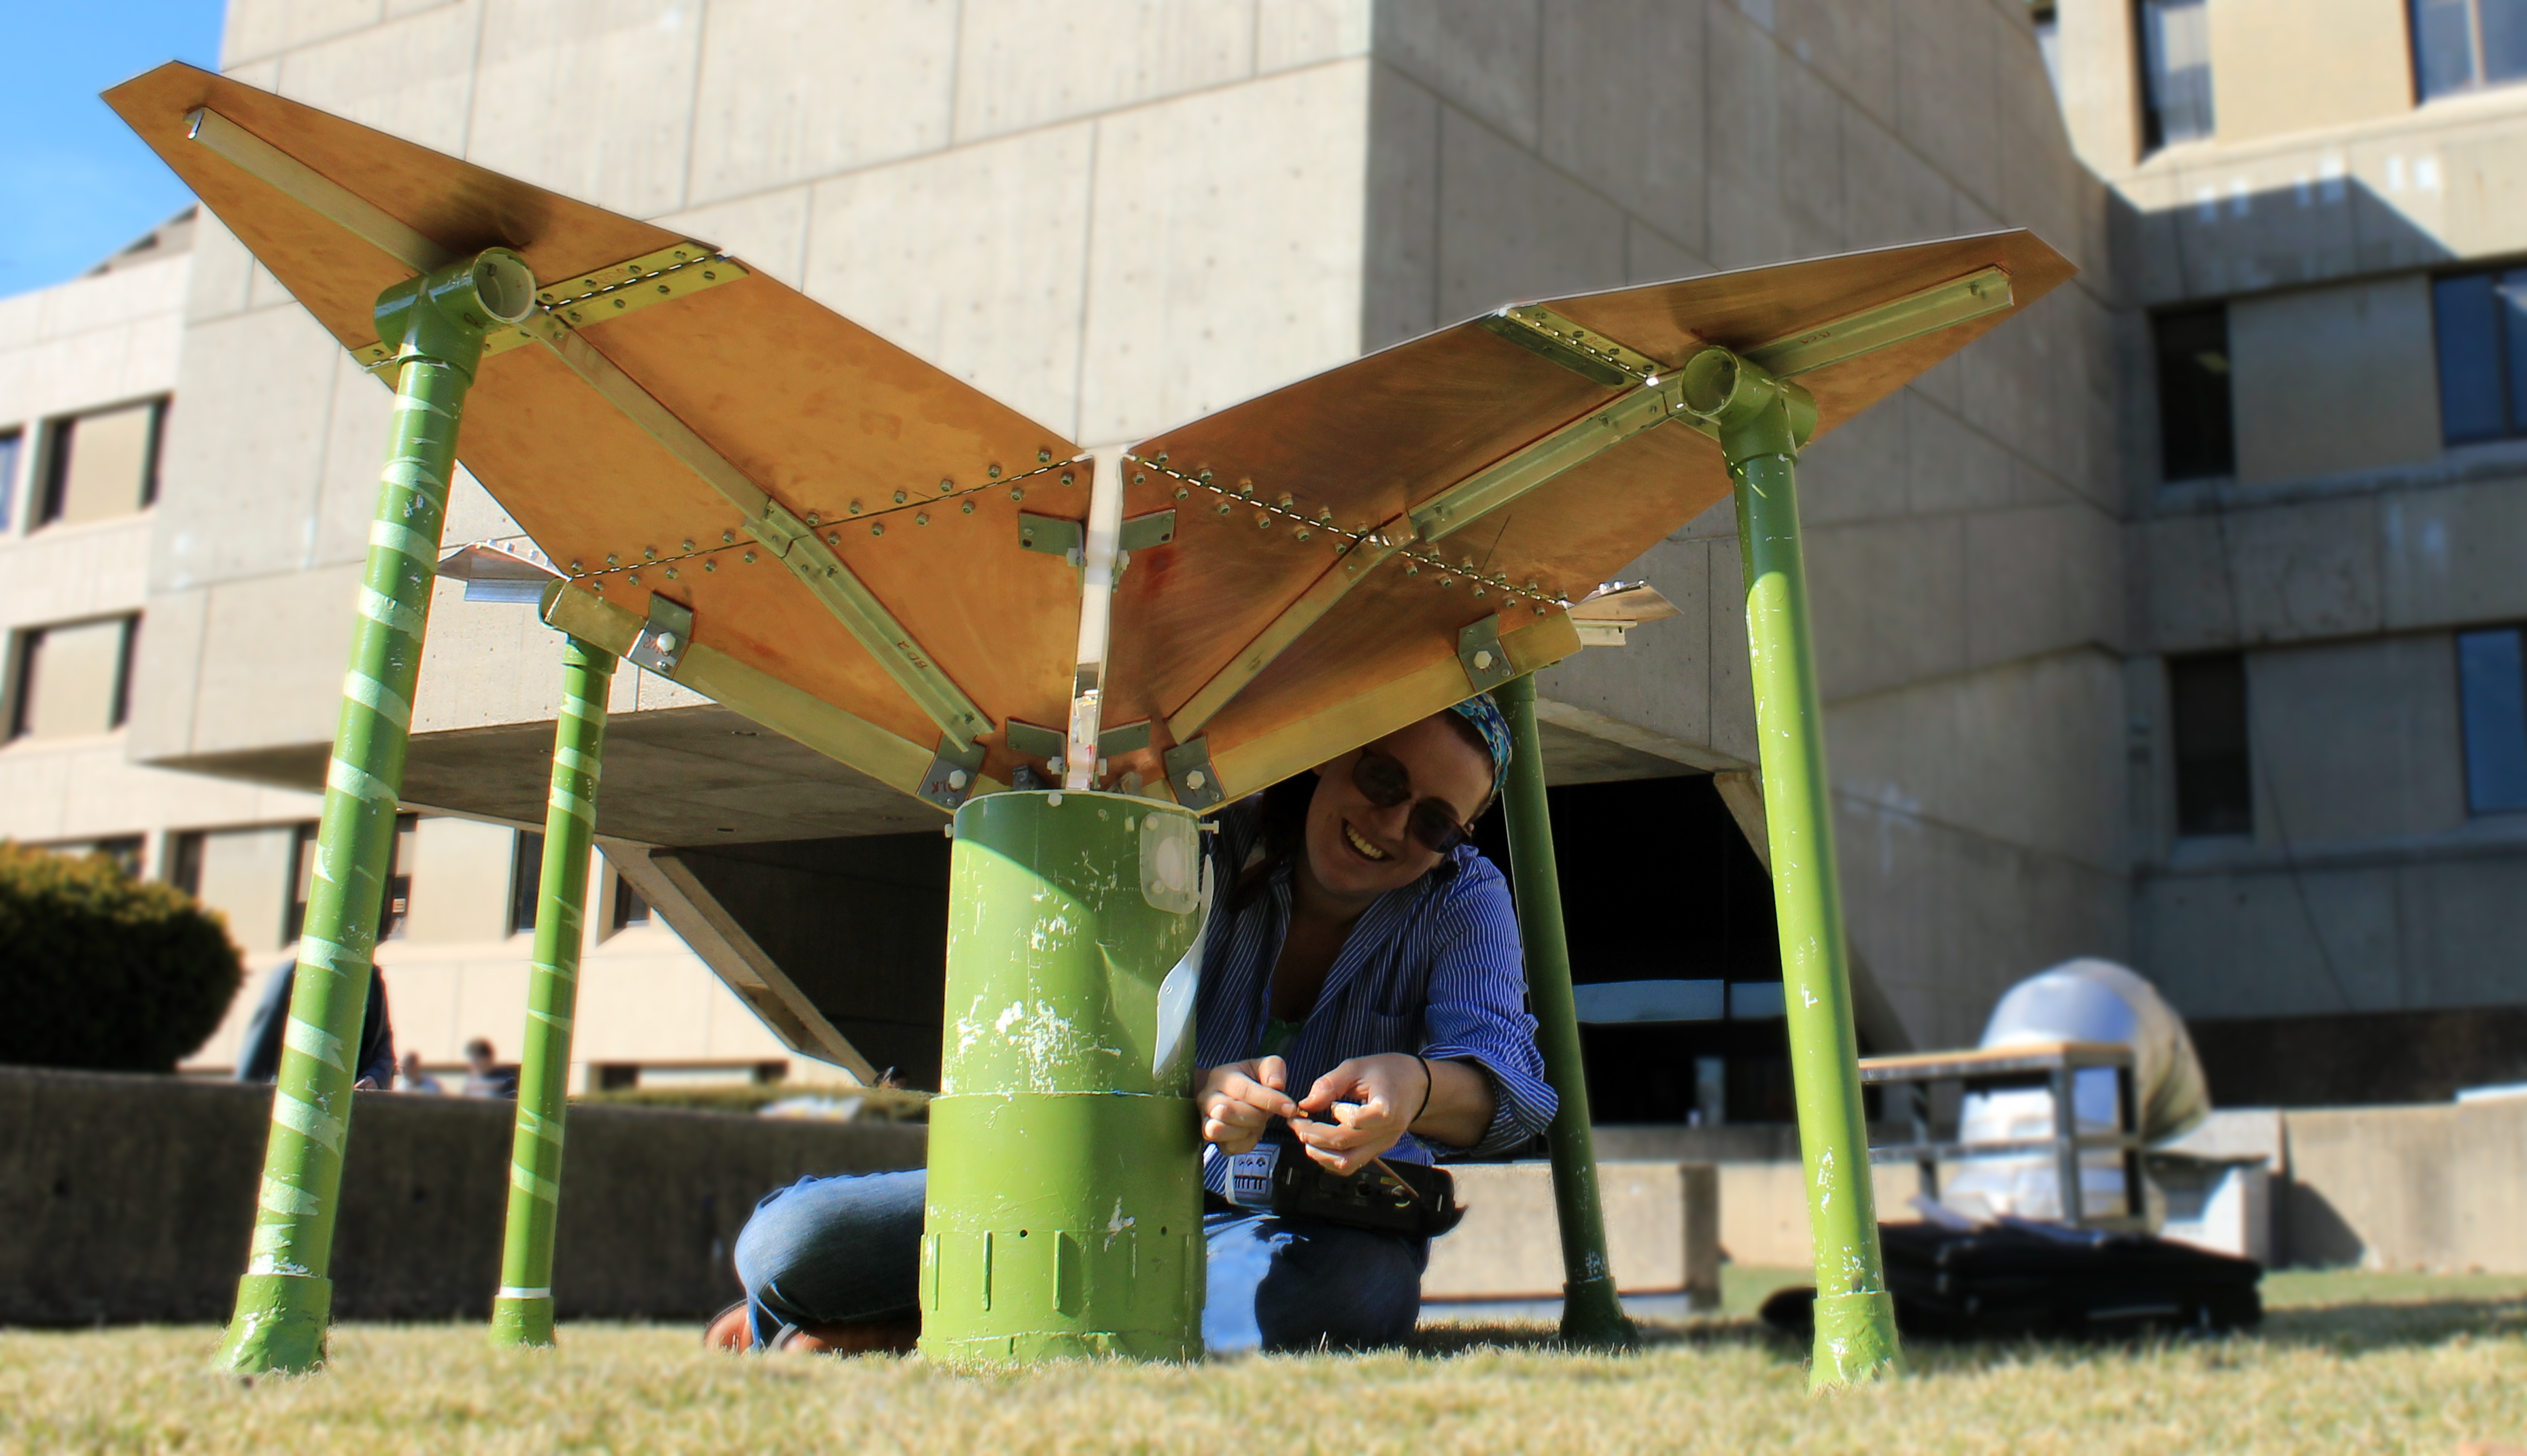
\includegraphics[width=0.95\linewidth]{SCIHI_system/figures/HIbiscus_100mhz.jpg}
\caption{New HIbiscus antenna scaled for 100 MHz as set up on the lawn at CMU while its S-parameters were measured. }
\label{Fig:hibiscus_100}
%\end{minipage}
\end{center}
\end{figure}

\subsubsection{Antenna Upgrades}
Deployment of the SCI-HI system in June 2013 demonstrated that the HIbiscus antenna could use some improvements prior to future deployements. The first and most significant change was the addition of a second antenna scaled to have a center frequency of 100 MHz. By having both scales (70 MHz and 100 MHz), data can now be collected over a wider range of frequencies. In addition, the overlap region where both antennas work ($\sim 85-95$ MHz) provides a cross check for the signal. In other words, this cross check will help us to make sure that any signal measured is not coming from the antenna structure. 

\begin{figure}[htb]
\centering
\begin{minipage}[b]{0.33\textwidth}
\centering
\includegraphics[width=0.95\linewidth]{SCIHI_system/figures/HIbiscus_petals.jpg}
\caption{HIbiscus petals with hinged joints.}
\label{Fig:hibiscus_petal}
\end{minipage}%
\begin{minipage}[b]{0.02\textwidth}
\hspace{1cm}
\end{minipage}%
\begin{minipage}[b]{0.61\textwidth}
\centering
\includegraphics[width=0.95\linewidth]{SCIHI_system/figures/HIbiscus_folded_70mhz.jpg}
\caption{HIbiscus petals folded up in preparation for packing.}
\label{Fig:hibiscus_fold}
\end{minipage}
\end{figure}

We built a new 70 MHz antenna (see Figure \ref{Fig:hibiscus_70}) as well as the 100 MHz antenna (see Figure \ref{Fig:hibiscus_100}) using the same shape as the original antenna. However, our deployment helped us to identify some changes to make to the physical construction of the antenna in order to make it easier to setup. We replaced the brass flanges that had to be screwed together to assemble each petal with hinged joints (made out of piano hinge) that do not have to be disassembled and reassembled (see Figure \ref{Fig:hibiscus_petal}). Figure \ref{Fig:hibiscus_fold} shows two of these petals when they are folded and stacked prior to being placed inside a bag for travel. 

In addition to the hinged joints, we also added extention pieces to the support PVC to allow us to use the same supports for both scaled versions of the antenna. This allowed us to add the second antenna with only one additional bag required for transport of both antennas compared to transport of just the 70 MHz antenna.  

\begin{figure}[htb]
\begin{center}
%\centering
%\begin{minipage}[b]{0.47\textwidth}
%\centering

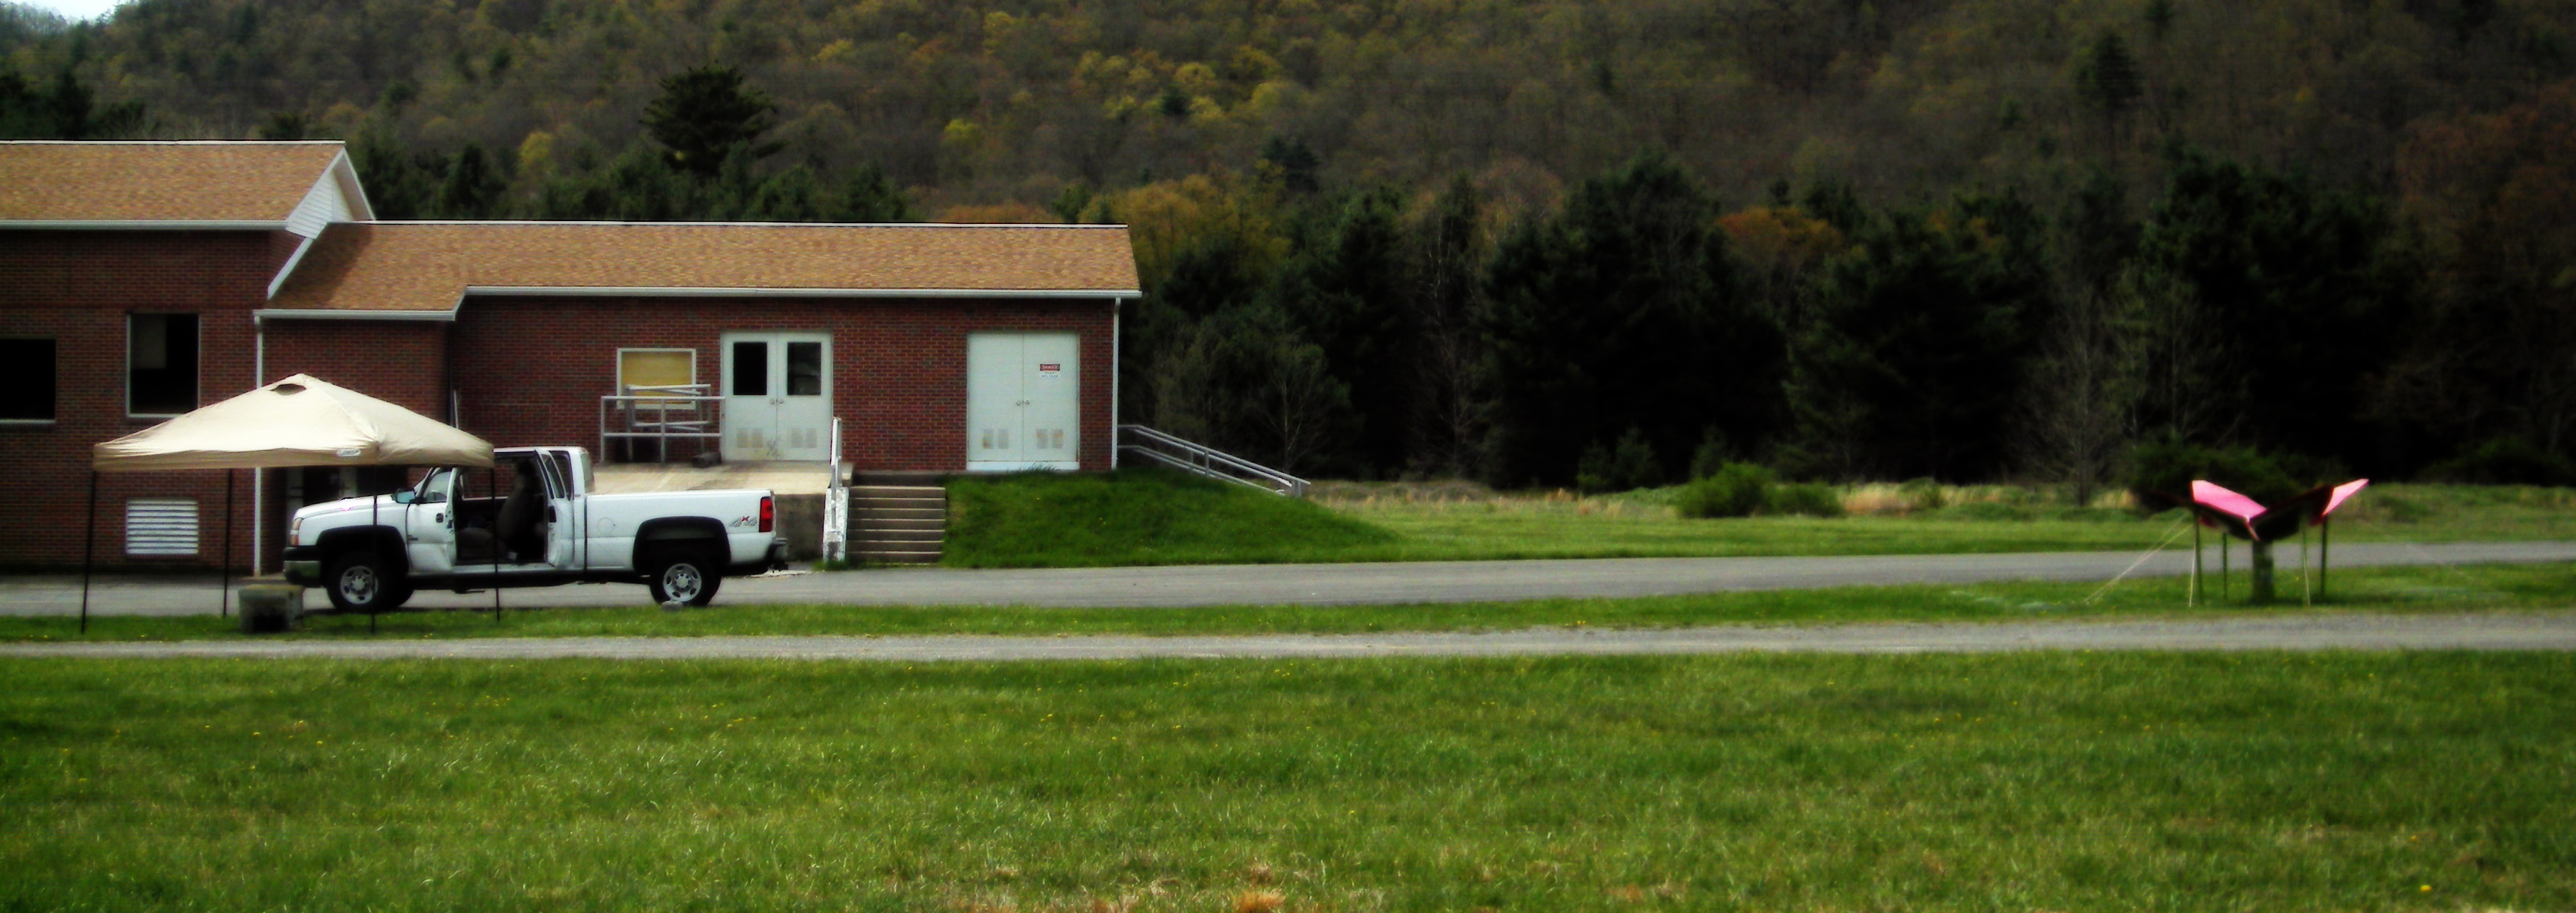
\includegraphics[width=0.95\linewidth]{SCIHI_system/figures/SCIHI_gbt_sys.jpg}
\caption{SCI-HI system with HIbiscus antenna set up on site at Green Bank in May 2013.}
\label{Fig:sys_gbt}

\end{center}
\end{figure}

%\end{minipage}%
%\begin{minipage}[b]{0.02\textwidth}
%\hspace{1cm}
%\end{minipage}%
%\begin{minipage}[b]{0.47\textwidth}
%\centering

\begin{figure}[htb]
\begin{center}
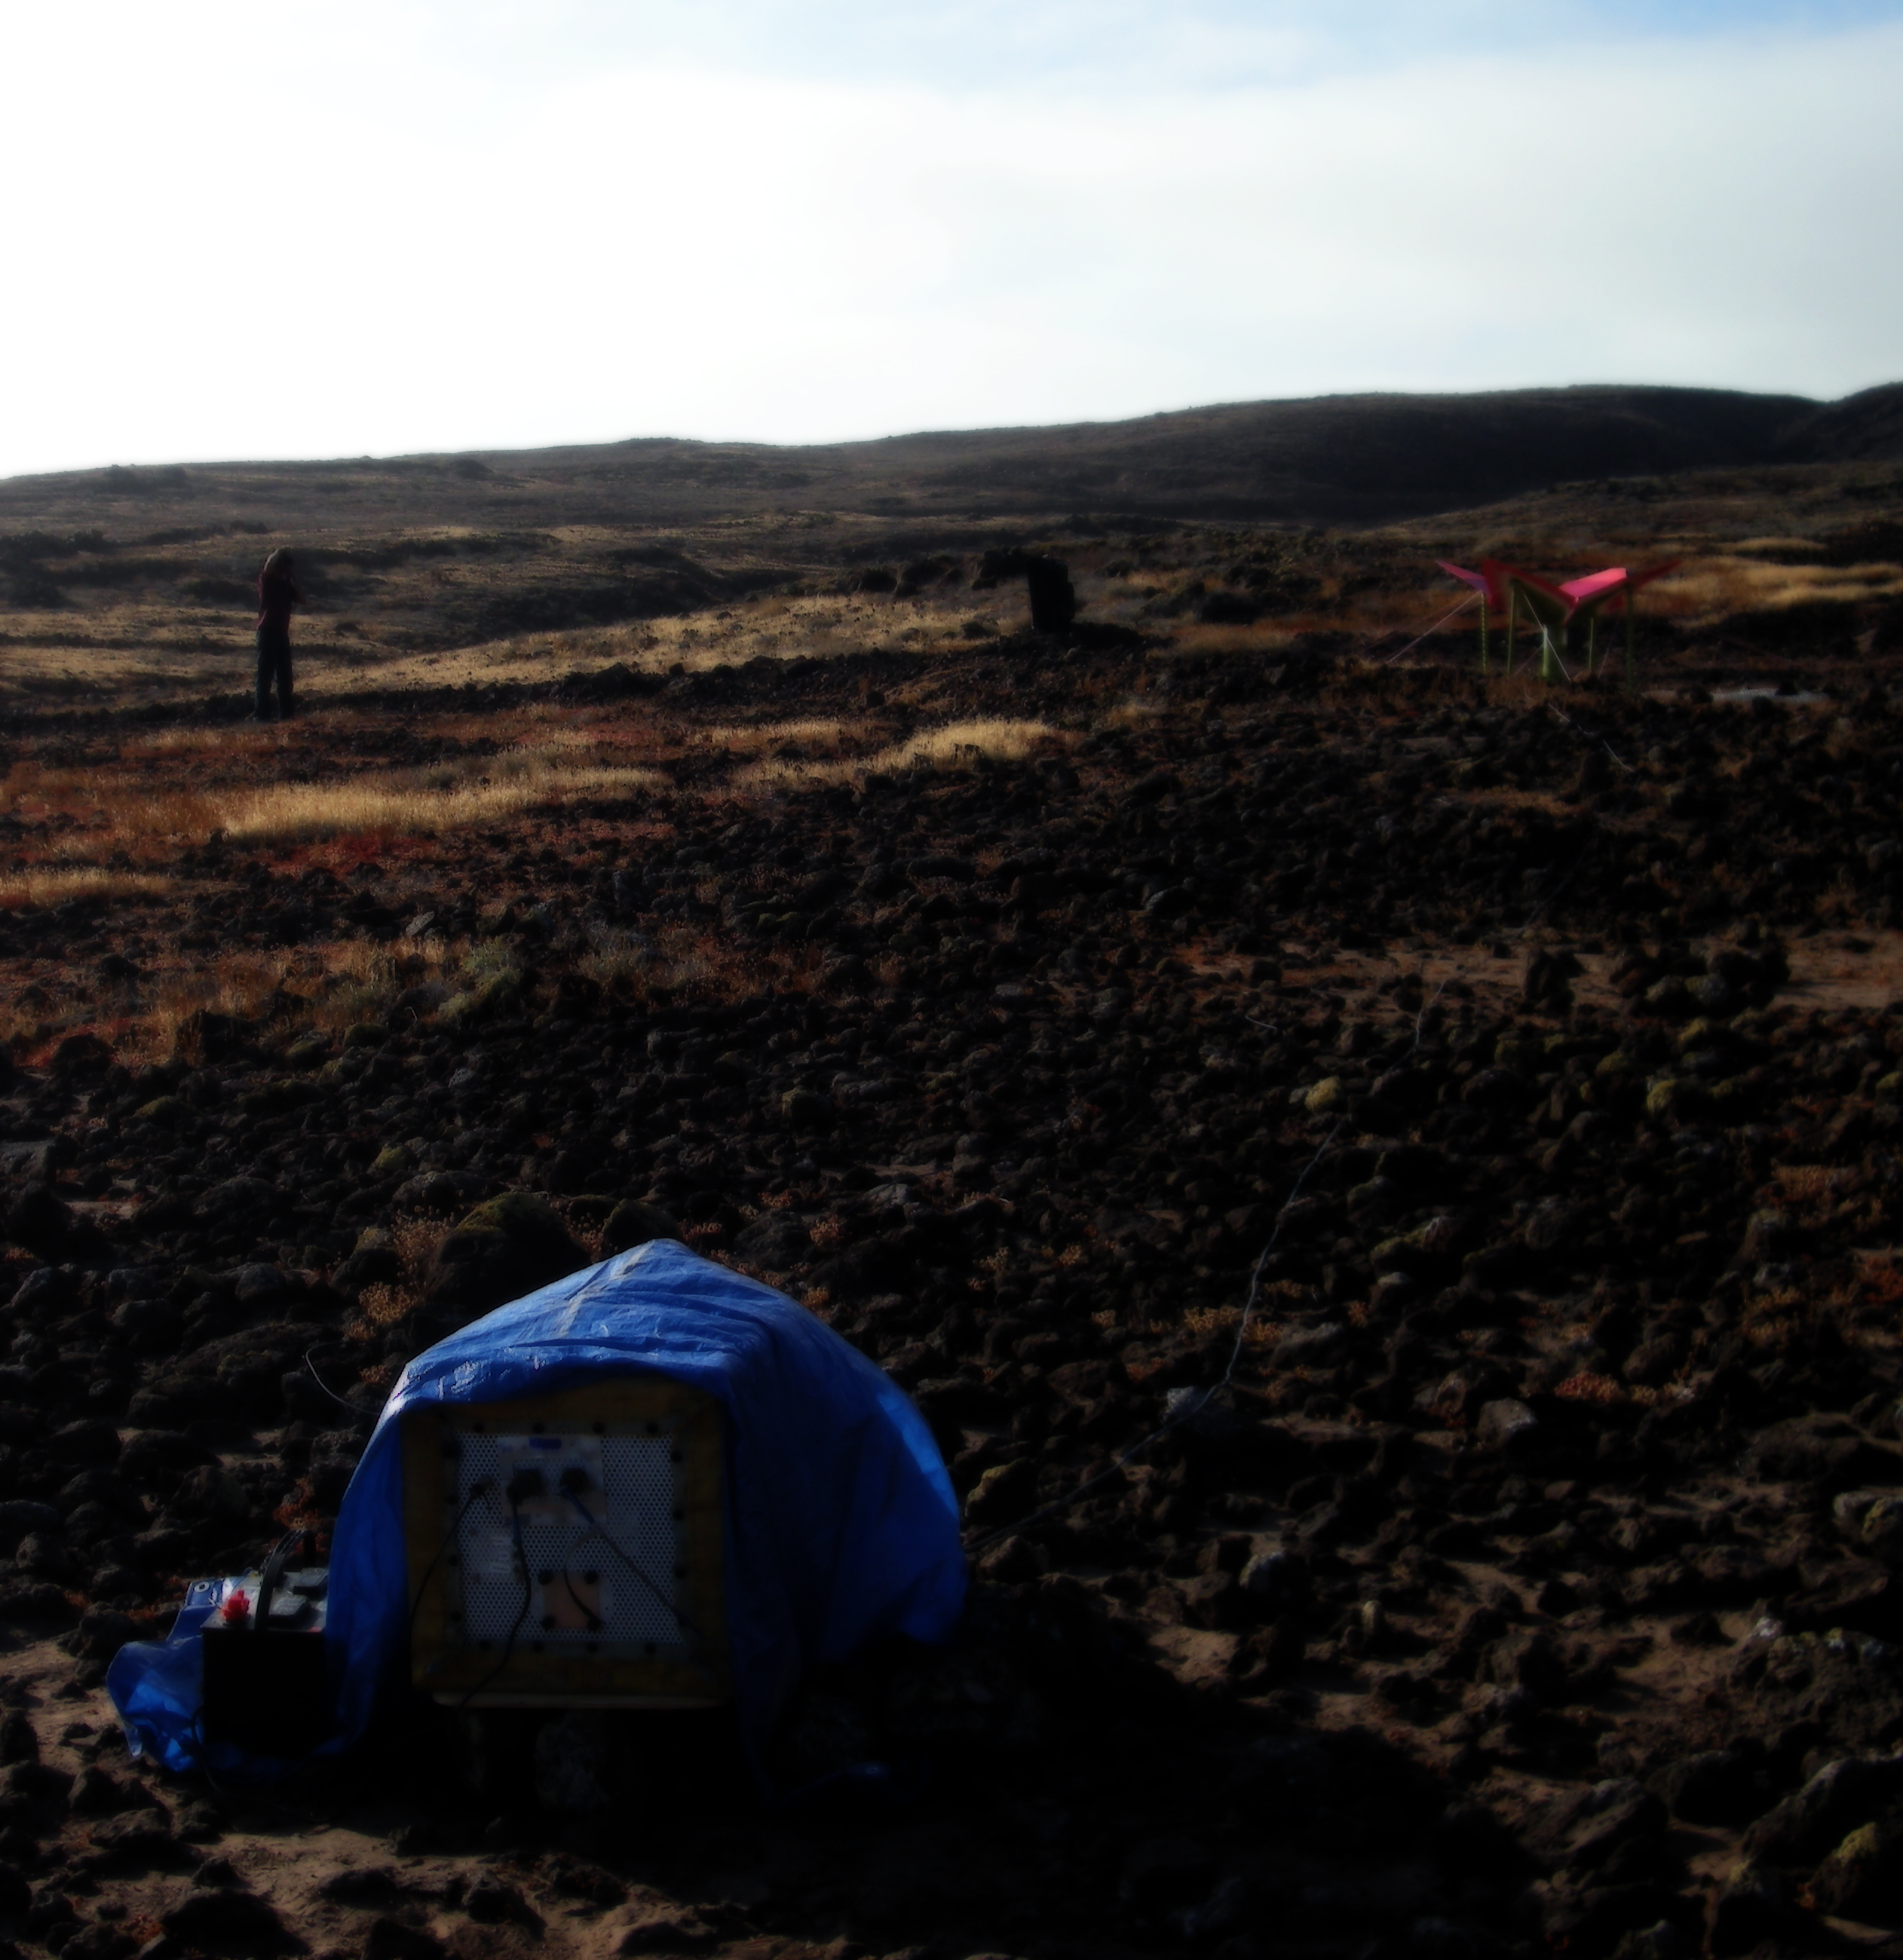
\includegraphics[width=0.95\linewidth]{SCIHI_system/figures/SCIHI_guad_sys.jpg}
\caption{SCI-HI system with HIbiscus antenna set up on site at Isla Guadalupe in June 2013}
\label{Fig:sys_guad}
%\end{minipage}

\end{center}
\end{figure}


\section{RF Electronics}

Once the signal from the sky has been collected by the antenna, it has to be transmitted to the data proccessing system in a form that the system is capable of processing. Transmission happens along a chain of radio frequency (RF) electronics. 

\textcolor{red}{Add a second level RF chain flow chart here.}
\subsection{RF Chain Overview}
For the SCI-HI system, the RF chain components are a switch, amplifiers, high and low pass filters, attenuators and a power splitter (along with the attendant cabling). Each of these components serves a specific purpose in the system. 

We can divide the RF chain into two sections based upon physical location. The first section is the antenna electronics, which sit as close to the antenna terminal as physically possible. The second section is the Faraday cage electronics, which sit next to the data processing system within a Faraday Cage. Between the two sections is a long signal cable ($\sim50-100 m$), allowing the antenna and data processing system to be placed far enough apart that the transmission of self-generated noise from the data processor is minimized (see Figures \ref{Fig:sys_gbt} and \ref{Fig:sys_guad}).

\begin{figure}[htb]
\centering
\begin{minipage}[b]{0.47\textwidth}
\centering
\includegraphics[width=0.95\linewidth]{SCIHI_system/figures/trombone_sys_switch.jpg}
\caption{Trombone antenna setup with calibration switch mounted directly below the antenna.}
\label{Fig:trombone_switch}
\end{minipage}%
\begin{minipage}[b]{0.02\textwidth}
\hspace{1cm}
\end{minipage}%
\begin{minipage}[b]{0.47\textwidth}
\centering
\includegraphics[width=0.95\linewidth]{SCIHI_system/figures/SCIHI_rf_ant_lower.jpg}
\caption{RF electronics box at the base of the trombone antenna with second stage amplifier and filters.}
\label{Fig:trombone_base}
\end{minipage}
\end{figure}

\textcolor{red}{Add a third level RF chain flow chart of just the antenna electronics here.}

\subsection{Antenna Electronics}
The antenna electronics are a calibration switch with known signal sources on some of the terminalsand two stages of amplification. In some versions of the electronics system, at least one of the RF filters was placed at the antenna end of the system but we'll discuss that component in the Faraday Cage electronics section. 

\subsubsection{Calibration Switch}
Because the SCI-HI system has a single antenna with a relatively large beam ($\sim 55^\circ$), calibrating the data from the antenna can be difficult. One way to do this calibration is to use noise source of known temperature whose signal is sent through the same RF chain as the antenna data (see Chapter \ref{Ch:Data}). 

In order to facilitate this calibration, a switch was placed at the terminal of the antenna. By making the antenna one of the inputs of the switch and matching one or more known temperature sources to the other switch inputs, data can be collected for all inputs with the same RF chain. 

We used a 6 input electromechanical switch (\textcolor{red}{Add part numbers here}) for the system. One input to the switch was connected directly to the antenna (see Figures \ref{Fig:trombone_switch} and \ref{Fig:rf_ant_mount}). The other inputs were a short terminator, a $50 \Omega$ load terminatore, a $100 \Omega$ load terminator, and an artificial noise source of known power. One input was left open. 

Switching between inputs is controlled through a cable from the Faraday Cage that carries both the power for the antenna electronics and the control signal. In addtion, the artificial noise source is turned off when that input is not enabled (to avoid noise bleeding into the antenna). We also built a manual switch control box that can be hooked up to the switch for testing. 

\begin{figure}[htb]
\centering
\begin{minipage}[b]{0.47\textwidth}
\centering
\includegraphics[width=0.95\linewidth]{SCIHI_system/figures/SCIHI_rf_ant_box.jpg}
\caption{New lucite box containing all the antenna RF electronics.}
\label{Fig:rf_ant_box}
\end{minipage}%
\begin{minipage}[b]{0.02\textwidth}
\hspace{1cm}
\end{minipage}%
\begin{minipage}[b]{0.47\textwidth}
\centering
\includegraphics[width=0.95\linewidth]{SCIHI_system/figures/SCIHI_rf_ant_box_mount.jpg}
\caption{RF electronics box attached to one of the HIbiscus antenna center mounts.}
\label{Fig:rf_ant_mount}
\end{minipage}
\end{figure}

\subsubsection{Amplifiers}
Immediatelly following the switch in the RF chain is the first stage amplifier. 

\textcolor{red}{Add general discussion of S-parameters and Transmission Efficiency followed by a section on the different types of amplifiers that we tried and why we selected the one that we did.}

\paragraph{S-parameters}

\paragraph{Transmission Efficiency}

\paragraph{Amplifier Selection}

\paragraph{Multi-stage Amplification}
Because the $\sim50-100 m$ signal cable will attenuate signals travelling down its length, a second stage amplifier was added to the system to increase the gain of the signal. Both amplifiers use DC power supplied by the same power cable as the switch. Because different levels of DC power were needed for the varying electronic components, voltage regulation circuits were also included in the antenna electronics housing. 

To maintain transmission efficiency, the first and second stage amplifiers' impedence had to match well. This was accomplished by using the same amplifier type for both stages. Initially the second stage amplifier was placed at the base of antenna (see Figure \ref{Fig:trombone_base}). However, this placement resulted in reflections in the signal whose period corresponded to the cable length between the two amplifiers. \textcolor{red}{May try to make a plot that shows this.} Therefore, the second stage amplifier was moved to a position immediately following the first stage amplifier (see Figure \ref{Fig:rf_ant_box}), which removed the effect. 

\begin{figure}[htb]
\centering
\begin{minipage}[b]{0.50\textwidth}
\centering
\includegraphics[width=0.95\linewidth]{SCIHI_system/figures/SCIHI_fcage_old.jpg}
\caption{Faraday cage around data processing system as setup in October 2012.}
\label{Fig:fcage_old}
\end{minipage}%
\begin{minipage}[b]{0.02\textwidth}
\hspace{1cm}
\end{minipage}%
\begin{minipage}[b]{0.44\textwidth}
\centering
\includegraphics[width=0.95\linewidth]{SCIHI_system/figures/SCIHI_filter.jpg}
\caption{Power signal filter box for one of the Faraday Cages.}
\label{Fig:fcage_filter}
\end{minipage}
\end{figure}

\begin{figure}[htb]
\centering
\begin{minipage}[b]{0.43\textwidth}
\centering
\includegraphics[width=0.95\linewidth]{SCIHI_system/figures/SCIHI_fcage_int.jpg}
\caption{Faraday cage around data processing system as setup in June 2013.}
\label{Fig:fcage_int}
\end{minipage}%
\begin{minipage}[b]{0.02\textwidth}
\hspace{1cm}
\end{minipage}%
\begin{minipage}[b]{0.51\textwidth}
\centering
\includegraphics[width=0.95\linewidth]{SCIHI_system/figures/SCIHI_fcage_new.jpg}
\caption{New Faraday Cage with double shielding around data processing system.}
\label{Fig:fcage_new}
\end{minipage}
\end{figure}

\subsection{Faraday Cage Electronics}

\subsubsection{Faraday Cage Design}

\subsubsection{Power Filters}

\subsubsection{RF Filters and Amplification}

\subsubsection{RF Signal Splitting}



\section{Data Processing}

\subsection{Overview}

\begin{figure}[htb]
\centering
\begin{minipage}[b]{0.54\textwidth}
\centering
\includegraphics[width=0.95\linewidth]{SCIHI_system/figures/SCIHI_comp.jpg}
\caption{Current version of the data processing system assembled inside a Faraday Cage box.}
\label{Fig:new_comp}
\end{minipage}%
\begin{minipage}[b]{0.02\textwidth}
\hspace{1cm}
\end{minipage}%
\begin{minipage}[b]{0.40\textwidth}
\centering
\includegraphics[width=0.95\linewidth]{SCIHI_system/figures/SCIHI_water_cooling_pipe.jpg}
\caption{Part of the water cooling system for the data processing machine.}
\label{Fig:water_pipe}
\end{minipage}
\end{figure}

\subsection{Analog to Digital Conversion and Sample Interleaving}

\subsection{Fourier Transformation and Data Collection Efficiency}

\subsection{Power Suppy and Consumption}

\subsection{System Noise Generation}

\subsection{User interface and system control}

